% Options for packages loaded elsewhere
\PassOptionsToPackage{unicode}{hyperref}
\PassOptionsToPackage{hyphens}{url}
%
\documentclass[
  letterpaper,
  DIV=11,
  numbers=noendperiod]{scrartcl}

\usepackage{amsmath,amssymb}
\usepackage{setspace}
\usepackage{iftex}
\ifPDFTeX
  \usepackage[T1]{fontenc}
  \usepackage[utf8]{inputenc}
  \usepackage{textcomp} % provide euro and other symbols
\else % if luatex or xetex
  \usepackage{unicode-math}
  \defaultfontfeatures{Scale=MatchLowercase}
  \defaultfontfeatures[\rmfamily]{Ligatures=TeX,Scale=1}
\fi
\usepackage{lmodern}
\ifPDFTeX\else  
    % xetex/luatex font selection
\fi
% Use upquote if available, for straight quotes in verbatim environments
\IfFileExists{upquote.sty}{\usepackage{upquote}}{}
\IfFileExists{microtype.sty}{% use microtype if available
  \usepackage[]{microtype}
  \UseMicrotypeSet[protrusion]{basicmath} % disable protrusion for tt fonts
}{}
\makeatletter
\@ifundefined{KOMAClassName}{% if non-KOMA class
  \IfFileExists{parskip.sty}{%
    \usepackage{parskip}
  }{% else
    \setlength{\parindent}{0pt}
    \setlength{\parskip}{6pt plus 2pt minus 1pt}}
}{% if KOMA class
  \KOMAoptions{parskip=half}}
\makeatother
\usepackage{xcolor}
\setlength{\emergencystretch}{3em} % prevent overfull lines
\setcounter{secnumdepth}{5}
% Make \paragraph and \subparagraph free-standing
\ifx\paragraph\undefined\else
  \let\oldparagraph\paragraph
  \renewcommand{\paragraph}[1]{\oldparagraph{#1}\mbox{}}
\fi
\ifx\subparagraph\undefined\else
  \let\oldsubparagraph\subparagraph
  \renewcommand{\subparagraph}[1]{\oldsubparagraph{#1}\mbox{}}
\fi


\providecommand{\tightlist}{%
  \setlength{\itemsep}{0pt}\setlength{\parskip}{0pt}}\usepackage{longtable,booktabs,array}
\usepackage{calc} % for calculating minipage widths
% Correct order of tables after \paragraph or \subparagraph
\usepackage{etoolbox}
\makeatletter
\patchcmd\longtable{\par}{\if@noskipsec\mbox{}\fi\par}{}{}
\makeatother
% Allow footnotes in longtable head/foot
\IfFileExists{footnotehyper.sty}{\usepackage{footnotehyper}}{\usepackage{footnote}}
\makesavenoteenv{longtable}
\usepackage{graphicx}
\makeatletter
\def\maxwidth{\ifdim\Gin@nat@width>\linewidth\linewidth\else\Gin@nat@width\fi}
\def\maxheight{\ifdim\Gin@nat@height>\textheight\textheight\else\Gin@nat@height\fi}
\makeatother
% Scale images if necessary, so that they will not overflow the page
% margins by default, and it is still possible to overwrite the defaults
% using explicit options in \includegraphics[width, height, ...]{}
\setkeys{Gin}{width=\maxwidth,height=\maxheight,keepaspectratio}
% Set default figure placement to htbp
\makeatletter
\def\fps@figure{htbp}
\makeatother
\newlength{\cslhangindent}
\setlength{\cslhangindent}{1.5em}
\newlength{\csllabelwidth}
\setlength{\csllabelwidth}{3em}
\newlength{\cslentryspacingunit} % times entry-spacing
\setlength{\cslentryspacingunit}{\parskip}
\newenvironment{CSLReferences}[2] % #1 hanging-ident, #2 entry spacing
 {% don't indent paragraphs
  \setlength{\parindent}{0pt}
  % turn on hanging indent if param 1 is 1
  \ifodd #1
  \let\oldpar\par
  \def\par{\hangindent=\cslhangindent\oldpar}
  \fi
  % set entry spacing
  \setlength{\parskip}{#2\cslentryspacingunit}
 }%
 {}
\usepackage{calc}
\newcommand{\CSLBlock}[1]{#1\hfill\break}
\newcommand{\CSLLeftMargin}[1]{\parbox[t]{\csllabelwidth}{#1}}
\newcommand{\CSLRightInline}[1]{\parbox[t]{\linewidth - \csllabelwidth}{#1}\break}
\newcommand{\CSLIndent}[1]{\hspace{\cslhangindent}#1}

\usepackage{booktabs}
\usepackage{longtable}
\usepackage{array}
\usepackage{multirow}
\usepackage{wrapfig}
\usepackage{float}
\usepackage{colortbl}
\usepackage{pdflscape}
\usepackage{tabu}
\usepackage{threeparttable}
\usepackage{threeparttablex}
\usepackage[normalem]{ulem}
\usepackage{makecell}
\usepackage{xcolor}
\KOMAoption{captions}{tableheading}
\usepackage[left]{lineno}
\linenumbers
\usepackage{xcolor}
\usepackage{caption}
\captionsetup[figure]{font=footnotesize}
\usepackage{float}
\floatplacement{table}{H}
\makeatletter
\makeatother
\makeatletter
\makeatother
\makeatletter
\@ifpackageloaded{caption}{}{\usepackage{caption}}
\AtBeginDocument{%
\ifdefined\contentsname
  \renewcommand*\contentsname{Table of contents}
\else
  \newcommand\contentsname{Table of contents}
\fi
\ifdefined\listfigurename
  \renewcommand*\listfigurename{List of Figures}
\else
  \newcommand\listfigurename{List of Figures}
\fi
\ifdefined\listtablename
  \renewcommand*\listtablename{List of Tables}
\else
  \newcommand\listtablename{List of Tables}
\fi
\ifdefined\figurename
  \renewcommand*\figurename{Figure}
\else
  \newcommand\figurename{Figure}
\fi
\ifdefined\tablename
  \renewcommand*\tablename{Table}
\else
  \newcommand\tablename{Table}
\fi
}
\@ifpackageloaded{float}{}{\usepackage{float}}
\floatstyle{ruled}
\@ifundefined{c@chapter}{\newfloat{codelisting}{h}{lop}}{\newfloat{codelisting}{h}{lop}[chapter]}
\floatname{codelisting}{Listing}
\newcommand*\listoflistings{\listof{codelisting}{List of Listings}}
\makeatother
\makeatletter
\@ifpackageloaded{caption}{}{\usepackage{caption}}
\@ifpackageloaded{subcaption}{}{\usepackage{subcaption}}
\makeatother
\makeatletter
\@ifpackageloaded{tcolorbox}{}{\usepackage[skins,breakable]{tcolorbox}}
\makeatother
\makeatletter
\@ifundefined{shadecolor}{\definecolor{shadecolor}{rgb}{.97, .97, .97}}
\makeatother
\makeatletter
\makeatother
\makeatletter
\makeatother
\ifLuaTeX
  \usepackage{selnolig}  % disable illegal ligatures
\fi
\IfFileExists{bookmark.sty}{\usepackage{bookmark}}{\usepackage{hyperref}}
\IfFileExists{xurl.sty}{\usepackage{xurl}}{} % add URL line breaks if available
\urlstyle{same} % disable monospaced font for URLs
\hypersetup{
  pdftitle={The Influence of Fluvial and Glacial Watershed Dynamics on Holocene Sediment Accumulation in Cariboo Lake, Columbia Mountains, British Columbia, Canada},
  pdfauthor={A. Cebulski \& J. Desloges},
  hidelinks,
  pdfcreator={LaTeX via pandoc}}

\title{The Influence of Fluvial and Glacial Watershed Dynamics on
Holocene Sediment Accumulation in Cariboo Lake, Columbia Mountains,
British Columbia, Canada}
\author{A. Cebulski \& J. Desloges}
\date{December 19, 2023}

\begin{document}
\maketitle
\ifdefined\Shaded\renewenvironment{Shaded}{\begin{tcolorbox}[interior hidden, enhanced, boxrule=0pt, sharp corners, frame hidden, breakable, borderline west={3pt}{0pt}{shadecolor}]}{\end{tcolorbox}}\fi

\setstretch{1.5}
\begin{center}\rule{0.5\linewidth}{0.5pt}\end{center}

A. Cebulski\textsuperscript{1,2} (ORCID ID - 0000-0001-7910-5056)

J. Desloges\textsuperscript{2} (ORCID ID - 0000-0001-8446-3034)

\textsuperscript{1}Centre for Hydrology, University of Saskatchewan,
Canada

\textsuperscript{2}Department of Geography and Department of Earth
Sciences, University of Toronto, Canada

Corresponding Author: A. Cebulski, alexcebulski@gmail.com

\begin{center}\rule{0.5\linewidth}{0.5pt}\end{center}

\pagebreak

\textbf{Abstract:} Records of sedimentation collected from Cariboo Lake,
situated in the northern Columbia Mountains, British Columbia, Canada,
are analyzed to assess Holocene fluvial and glacial watershed dynamics.
The aim of this study is to provide a proxy record of Holocene
hydroclimate and glacier change from sediment archives at a higher
temporal resolution compared to available records for the Interior
Ranges of British Columbia. Deglacial and Holocene sediment accumulation
is observed to reach a maximum thickness of 35 m in deep parts of the
lake, using sub-bottom acoustic soundings. A transition from massive to
well-stratified sediments is observed in the sub-bottom acoustic record
during final phases of valley deglaciation in the region
(\textasciitilde10.5--9 cal ka BP). Laminae couplets are interpreted to
be deposited annually according to two \textsuperscript{14}C dates and a
varve counting chronology. Two long cores, 2.9 and 3.8 m in length, were
selected for analysis with estimated basal dates of 2 cal ka BP. Trends
in downcore sediment characteristics were linked to environmental
changes in the glaciated catchment headwaters at a temporal resolution
of \textasciitilde100 yrs. Upstream lake filtering of river floodplains
and lakes prevented finding a higher temporal resolution linkage between
the sediment characteristics and headwater fluvial and glacial activity.
Despite some upstream filtering, the Cariboo River was found to be the
primary source of sediment to the long core sites. Observed grain size
and varve thickness from two long cores show above average trends which
are coincident with cooler temperatures and the primary glacier advances
over the last 2 ka.

\textbf{Keywords:} Glaciolacustrine; Varve; Hydrology; Climate; British
Columbia; Holocene

\pagebreak

\hypertarget{introduction}{%
\section{Introduction}\label{introduction}}

Climatic variability in the western Canadian Cordillera over the
Holocene contributed to several fluctuations in glacial activity with
implications for sediment accumulation in glacier-fed lakes. There is
general regional agreement between the Coast Mountains (Brown et al.,
2006; Koch et al., 2007; Menounos et al., 2004; Menounos \& Clague,
2008; Osborn et al., 2007; Ryder \& Thomson, 1986) and Canadian Rocky
Mountains (Hodder et al., 2006; Leonard, 1997; Luckman, 1988, 1993;
Luckman et al., 1993) on the timing and magnitude of the large early
Holocene retreat and late Holocene advances. However, the smaller
fluctuations that occurred between these large events have less regional
agreement (Menounos et al., 2009). Furthermore, few proxy records exist
in central British Columbia, that provide a high-resolution record of
Holocene hydroclimatic variability (Gilbert \& Desloges, 2012; Hodder et
al., 2006; Maurer et al., 2012; Menounos et al., 2009). Central British
Columbia is characterized by a transitional climate between the wetter
Coast Mountain Ranges to the dryer Rocky Mountain Ranges, which may
contribute to a different response of glaciers for this region over the
Holocene.

A study by Gilbert \& Desloges (2012) of Quesnel Lake (272
km\textsuperscript{2}), 30 km south of the study area examined here,
found high rates of sediment accumulation around 10.4 cal ka BP during
early Holocene deglaciation, and around 8.4 cal ka BP sediment
accumulation declined significantly. Meaningful trends in organic matter
and grain size of Quesnel Lake sediment sequences at a sub-millennial
time scale were not detectable. Quesnel Lake is very large relative to
the contributing watershed and therefore the sediment system exhibits
very low accumulation rates and is much less sensitive to climate
variability. Within the Cariboo Lake basin, Maurer et al. (2012)
investigated the headwater On-off Lake which remained intermittently
connected to the Castle Creek Glacier on the basin divide
(Figure~\ref{fig-map-basin}). Currently the Castle Creek Glacier resides
outside of the Cariboo Lake basin, however, Maurer et al. (2012) show
that the glacier advanced north across the hydrological divide and into
the Cariboo Lake basin several times over the Holocene. Both Gilbert \&
Desloges (2012) and Maurer et al. (2012) provide a long-term but coarse
temporal resolution record of Holocene hydroclimatic variability in the
Cariboo Mountains. Additional high-resolution proxy records of Holocene
fluvial and glacial activity are needed for this transitional climate of
central British Columbia; especially for the mid to late Holocene
interval where greater regional variability in glacial responses to
climate change has been observed (Menounos et al., 2009).

Environmental proxy records that extend back beyond the modern
observable record are crucial to understanding earth system processes
(Huber \& Knutti, 2012; Nelson et al., 2016; Turney et al., 2019). Proxy
reconstructions at the sub-annual (e.g., ice cores, tree rings, corals,
varved-sediments), to multi-decadal scales (e.g., sediments, pollen,
boreholes) have proven useful in describing past environmental
conditions across the globe (Masson-Delmotte et al., 2013). In the case
of sedimentary sequences collected from climate sensitive glaciated
watersheds, they have been important in contributing to the regional
understanding of climate and hydrologic variability over the Holocene.
For example, researchers have utilized sedimentary sequences along with
other environmental archives to provide regional (Menounos et al., 2009)
and global (Neukom et al., 2019) reconstructions of glacier and
hydroclimatic change over the Holocene. The sensitivity and temporal
resolution of lake sediment characteristics (e.g., varve thickness,
grain size and organic content) and their connection to regional
hydrology, temperature, precipitation patterns, and glacier extent
varies amongst glacier-fed lake studies (Desloges, 1999; Hodder et al.,
2006; Leonard, 1997; Menounos, 2006; Menounos \& Clague, 2008). Mountain
basins that exhibit a strong nival-hydrographic regime typically produce
distinct varve couplets with a fine-grained layer deposited in winter
when the lake ices over and turbulence decreases followed by a
coarse-grained layer deposited during spring high flows (e.g., Desloges,
1999; Hodder et al., 2007; Leonard, 1997). In contrast, lakes proximal
to the Coast Mountains of British Columbia may have multiple coarse
laminations within a single season due to the influence of frequent and
large fall rainstorms or mid-winter melt events (e.g., Gilbert et al.,
1997; Menounos \& Clague, 2008). Establishing a correlation between
seasonal or annual trends in sediment core varve thickness, grain size,
and organic content with local discharge, temperature, and precipitation
is not always possible due to complex process interactions, watershed
connectivity and dating uncertainties (Heideman et al., 2018; Hodder et
al., 2007; Menounos \& Clague, 2008). The linkage between hydrology and
climate drivers and the lake sediment record may be limited at short
time scales (i.e., less than 10 years) if there is weak connectivity
between sediment production and delivery to the lake (Heideman et al.,
2018; Hodder et al., 2007; Menounos \& Clague, 2008). Trends in lake
sediment sequences are typically more representative of climate
fluctuations at time scales greater than 100 years as this provides
sufficient time for changes in sediment production and delivery to
propagate through the watershed (Heideman et al., 2018; Leonard \&
Reasoner, 1999; Osborn et al., 2007).

The purpose of this research is to 1) establish an understanding of the
mechanisms that control the delivery and deposition of the fine sediment
fraction to Cariboo Lake, 2) to reconstruct the highest resolution and
longest possible sediment accumulation record from cores and acoustic
methods for this semi-arid region of British Columbia, 3) determine if
the sediment accumulation record contains a signal from fluvial and
glacial activity driven by regional to continental hydroclimate change,
and 4) ascertain how this record of hydroclimatic variability differs
from other records collected in the Coastal and Rocky Mountains.

\hypertarget{materials-and-methods}{%
\section{Materials and methods}\label{materials-and-methods}}

\hypertarget{study-area}{%
\subsection{Study Area}\label{study-area}}

Cariboo Lake is located in the northern foothills of the Columbia
Mountains, 85 km northeast of Williams Lake, British Columbia
(Figure~\ref{fig-map-basin}). The lake is separated into two basins by a
large alluvial fan building cross-valley from Keithley Creek
(Figure~\ref{fig-map-lake}). The main Cariboo Lake basin, to the
northeast of Keithley Creek, receives discharge from an area of 2636
km\textsuperscript{2}, which is filtered by three upper watershed lakes:
Issac Lake, Lanezi Lake, and Ghost Lake (Figure~\ref{fig-map-basin}).
While lakes proximal to glacial activity may contain sediment archives
more closely linked to headwater changes in fluvial and glacial
activity, their higher sediment accumulation rates and remote location
would have made it very difficult to retrieve a long-term sediment
record. Due to the upstream filtering effect from these upvalley lakes,
Cariboo Lake has a lower sediment accumulation rate, presenting a more
accessible option to retrieve a sediment record spanning a longer time
interval.

The watershed relief ranges from 2600 m in the eastern Cariboo Mountain
headwaters to 600 m at the western Cariboo Lake outlet. The lake area to
watershed area ratio of the main Cariboo Lake basin is 0.3\%. The
southwest to northeast, 75 km long watershed spans a precipitation
gradient ranging from 1370 mm yr\textsuperscript{-1} in the headwaters
to 477 mm yr\textsuperscript{-1} at the semi-arid outlet to the lake.
The Cariboo Lake watershed has 75 km\textsuperscript{2} of permanent ice
cover which covers 3\% of the total watershed (Bolch, 2008). The most
extensive glaciated terrain is proximal to Mt. Lunn roughly 60 km
upstream of Cariboo Lake (Figure~\ref{fig-map-basin}). The Cariboo Lake
basin hydrology is inferred from the Water Survey of Canada station
08KH003 (Albers, 2017) 20 km downvalley from the Cariboo Lake outlet
(Figure~\ref{fig-map-basin}). The watershed is snow- and glacier-melt
dominated with average 1971-2000 monthly runoff peaking in June (220 mm)
and low-flows that occur between December and March (15--25 mm)
(Figure~\ref{fig-cl-hydro}, A). From December to March air temperature
is mostly below 0 °C and precipitation falls primarily as snow
(Figure~\ref{fig-cl-hydro}). The bathymetry of the lake reaches a
maximum depth of just over 50 m in two deep holes within the central
part of the main Lake basin (Figure~\ref{fig-map-lake}).

Upper watershed Lanezi Lake and Sandy Lake contrast significantly in
maximum depths at 170 m and 6 m, respectively
(Figure~\ref{fig-map-basin}). The Matthews River, which meets the
Cariboo River below Lanezi Lake, is filtered by Ghost Lake and provides
an important connection to a large area of ice (10
km\textsuperscript{2}), proximal to Roberts Peak
(Figure~\ref{fig-map-basin}).

\hypertarget{field-methods}{%
\subsection{Field Methods}\label{field-methods}}

A field campaign was conducted during the summer of 2017 to collect
sub-bottom acoustic soundings, dredge samples, and sediment cores.
Thirty-four kilometres of sub-bottom acoustic soundings were collected
across Cariboo Lake using a 10 kHz StrataBox 3510 HD
(Figure~\ref{fig-map-lake}). Following a longitudinal transect down
Cariboo Lake, an Ekman dredge was used to collect 20 samples, each
yielding \textasciitilde730 cm\textsuperscript{3} of surficial sediment
(Figure~\ref{fig-map-lake}). The dredge samples were sub-sampled in the
field using an 8 cm diameter PVC cylinder. This resulted in 20 short
cores each containing about 450 cm\textsuperscript{3} of sediment.
Sub-sampling the dredge samples allowed for better preservation of the
sediment stratigraphy and confidence in capturing the sediment surface.
The Ekman dredge cores ranged from 6--12 cm in length. The sediment not
captured in the PVC cylinder was kept as a bulk sediment sample.

Four long sediment cores (V1--V4) were collected using a Rossfelder
submersible vibracorer with a 6 m long, 6 cm diameter, aluminum pipe
(Figure~\ref{fig-map-lake}). Sediment cores V1--V4 were retrieved at
deep mid-lake locations to ensure the cores consisted of a higher
fraction of fine clastic sediments. It was anticipated that the
transport of coarser-grained sediments from non-glaciated tributaries
would be limited to areas proximal to the lake's perimeter. Some
contribution of organic matter and clastic sediments to the long cores
from the smaller sidewall tributaries is anticipated. The extent of this
contribution was assessed using the Ekman surficial cores. While the top
and bottom of the long cores were sealed after retrieval, there is a
possibility of some sediment loss during the coring procedure and
transport. A gap of 3 m for V1 and 2 m for V2 between the top of the
retrieved sediment and the top of the coring tube helped minimize
sediment spillage from the top of the core during retrieval. Cores V1
and V2 in the Cariboo River basin were selected for detailed analysis as
these two cores had the highest fraction of fine clastic sediments,
their sediment stratigraphy was well preserved, and they both had
organic material for \textsuperscript{14}C dating. Cores V3 and V4 taken
closer to the Frank Creek and Keithley Creek deltas also had higher
fractions of coarse grained sediments and core disturbance and were not
analyzed in detail.

\hypertarget{laboratory-methods}{%
\subsection{Laboratory Methods}\label{laboratory-methods}}

Long and short cores were split longitudinally with one half preserved
as an archive and the other as a working half. The working half samples
were prepared for imaging by scraping the core parallel to the sediment
laminae to show the sediment stratigraphy. The short and long sediment
cores were analyzed for laminae thickness, organic content, and particle
size. The working halves of long cores V1 and V2 were subsampled with 2
cm\textsuperscript{3} of sediment extracted at a 5 cm interval, with
additional samples taken within stratigraphic facies that had visual
changes in grain size and lamination patterns. Laminae couplets observed
on the working halves were digitally counted and measured for thickness
using the ImageJ software (Schneider et al., 2012). The uncertainty of
the laminae counting in this study was inferred from Ekman short cores
(E12, E13, E14) which had statistically similar sediment accumulation
rates. The varve counting error was estimated by counting the number of
couplets down to a depth of 5 cm in each Ekman core. The top section of
cores V1 and V2 were disturbed during coring and transport which
prevented counting and measurement of laminae couplets in 11 cm of V1
and 7 cm of V2. The short core E13, with a depth of 8.8 cm, was used to
provide a sedimentation rate for the top sections of V1 and V2 with
indiscernible laminae. The absence of clear marker laminae limited the
confidence in anchoring of V1 and V2 to E13. To align cores V1 and V2
with E13 an age of 2017 (the year of core retrieval) was assigned to the
top of the cores. The confidence in the top of each core representing
the year of core retrieval relies on the assumption that no sediment was
lost from the top of the core during retrieval or transport.

Organic matter was approximated from percent weight loss-on-ignition
analysis (550 °C) (Dean, 1974; Smith, 2003). Grain size analysis was
conducted using a Mastersizer Particle Size Analyzer 3000. Samples were
prepared following methods by Gray et al. (2010) to remove organic
material. Three sequential aliquots of 20\%
H\textsubscript{2}0\textsubscript{2} were added until the sample stopped
reacting. To prevent flocculation of sediment grains the samples were
dispersed in 0.05\% solution of sodium hexametaphosphate for 24 hours.
Grain size was measured three times for each sample, resulting in an
average standard deviation of ± 0.01 µm.

The chronology of both long cores was reconstructed from Accelerator
Mass Spectrometry (AMS) \textsuperscript{14}C ages of organic material
(twigs and a conifer needle) found within the cores, and a chronology
derived from laminae couplet counting on working core images. The
\textsuperscript{14}C calibration was performed using Bchron, a Bayesian
statistical age-model software package for R (Haslett \& Parnell, 2008;
Parnell et al., 2008; Parnell et al., 2011) and the IntCal20 calibration
curve (Reimer, 2020). All data analysis and figures were produced using
the R language (R Core Team, 2022). Calibrated dates are reported as
thousands of years before 1950 (cal ka BP) or the number of years before
1950 (cal yr BP). Non calibrated dates are reported as the number of
years before 1950 (yr BP).

\hypertarget{results}{%
\section{Results}\label{results}}

\hypertarget{sub-bottom-acoustics}{%
\subsection{Sub-bottom Acoustics}\label{sub-bottom-acoustics}}

Acoustic stratigraphy from six Transects (Figure~\ref{fig-map-lake})
reveal the range of morphologies and character of infilling sedimentary
deposits in Cariboo Lake (Figure~\ref{fig-acoustics}). Acoustic
penetration is limited in Transects A and E by coarse sediments proximal
to river fan-deltas across Cariboo Lake (see triangle symbols in
Figure~\ref{fig-map-lake} for fan-delta locations). Acoustic signal
penetration, resolution and distinctive acoustic layering improves
significantly along the thalweg of the lake bottom away from the main
Cariboo River delta along Transects B, C, and D. In the Frank Creek and
Keithley Creek sub-basins acoustic penetration is reduced along Transect
E and F. The diagonal lines across all panels (cross-hatching) in
Figure~\ref{fig-acoustics} is observed over most of the acoustic record
due to errant electrical interference from the research vessel that
could not be resolved. However, the interference does not affect the
overall quality of the acoustic results in the six Transects
(Figure~\ref{fig-acoustics}).

Transect B, 3.5 km from the Cariboo River delta, has acoustic reflectors
with 1--2 m separation that lie conformably over a hummocky basement
(Figure~\ref{fig-acoustics}, B). The acoustic basement drops off below
the observable record near the south channel-like depression
(Figure~\ref{fig-acoustics}, B-Ae). Well-structured layering extends
across the south side of the Transect but pinches out towards the north
shore (Figure~\ref{fig-acoustics}). On the south side of Transect B, the
thickness of acoustically well-stratified deposits ranges from 10--20 m.

Acoustic penetration in the acoustic record increases 4.5 km from the
Cariboo River delta along Transect C, where the maximum sediment
thicknesses of 35 m are observed (Figure~\ref{fig-acoustics}, C). Two
sharp-crested v-shaped scour channels are observed in the middle of
Transect C (Figure~\ref{fig-acoustics}, C-Sc). The channels are the same
as those in Transect B (Figure~\ref{fig-acoustics}, B-Sc) and are
interpreted to be scour channels formed by erosive, high energy,
turbidity currents that eroded into coarse-grained glacial sediment
during the last deglaciation of the valley. Two sediment facies are
observed above the acoustic basement (Figure~\ref{fig-acoustics}, C-Ae)
based on geometry and the strength and continuity of reflectors. The
lower unit, Facies A, has a thickness of \textasciitilde12 m along on
the south sidewall of the transect (Figure~\ref{fig-acoustics}, C-FA)
and has a dominantly massive sediment structure. Facies A, is comprised
of a lighter grey tone representing coarse-grained sediment and lacks
parallel reflectors indicating a higher energy and more rapid deposition
of coarser lacustrine sediment. Facies B begins with high-amplitude
parallel reflectors with 2--3 m separation and conforms well with Facies
A below (Figure~\ref{fig-acoustics}, C-FA). Facies B has an average
thickness of \textasciitilde10 m and reaches a maximum thickness of 13 m
above the two scour channels (Figure~\ref{fig-acoustics}, C-Sc).

Transect D, to the northeast of the Frank Creek delta has well-layered
sediments in the top 5--10 m and transitions to poor acoustic
penetration below this (Figure~\ref{fig-acoustics}, D). The parallel
reflectors observed in the uppermost sediment layers of Transect D have
a thickness of 2--3 m and have a higher amplitude compared to Facies B
in Transect C. Some slumping of sidewall sediments is observed on the
south sidewall (Figure~\ref{fig-acoustics}, D-Sp).

\hypertarget{spatial}{%
\subsection{Spatial Trends in Surficial Sediment}\label{spatial}}

The surficial sediment cores show declining trends in grain size and
laminae thickness with distance from the main Cariboo River delta.
Trends in percent organic matter (OM) of surficial sediment cores were
not found to exhibit systematic patterns with distance down-lake
(Figure~\ref{fig-ekmanSeds}, C). The steep decline in grain size
suggests that larger sand-sized sediments (63--2000 µm) are sensitive to
distance from fan deltas, while smaller silt-sized (2--63 µm) and
clay-sized (0.01--2 µm) sediments are transported further down-lake. The
highest percent of silt (86.5--89.6\%) and clay (9.3--14.4\%) sized
sediments are observed between 3 and 6.5 km from the Cariboo River
delta, proximal to the long core sampling locations. Higher
D\textsubscript{50} grain size and percentage of sand sized grains were
also found proximal to the Frank Creek fan-delta and within the Keithley
Creek sub-basin (Figure~\ref{fig-ekmanSeds}, A \& B).

Proximal to the Cariboo River delta the structure of the surficial
sediments are dominantly massive, have erosive contacts and a fraction
of sand grains greater than 60\%. A sand-bed with a thickness of 1 cm
was observed in E1, the core closest to the Cariboo River delta
(Figure~\ref{fig-ekmanImgs}, A). In the main Cariboo River basin, core
E13, retrieved 5.24 km from the Cariboo River delta and from a depth of
40 m, contained fine, rhythmically laminated sediment
(Figure~\ref{fig-ekmanImgs}, B).

Sediment cores E9--E15 and E18--E20, retrieved from areas distal to the
main Cariboo River delta, at lake depths of 30--50 m, have a high
fraction of silt and clay sediment and exhibit a rhythmic sequence of
fine-grained dark layers overlain by coarse-grained light layers
(Figure~\ref{fig-ekmanImgs}, B \& C). The sediment stratigraphy observed
within cores E9--E15 and E18--E20 are similar to annual laminations
(varves), which occur in lakes that have sufficient seasonal variation
in river and sediment discharge as well as lake stratification
(Desloges, 1999; Smith \& Ashley, 1985; Zolitschka et al., 2015). In the
Cariboo Lake basin, winter low flows, lake-ice cover, and lake
stratification reduce the velocity of lake currents and contribute to
the deposition of normally graded fine-grained sediments on the lake
bottom. During spring snowmelt high flows, coarser-grained sediments are
deposited from higher energy lake currents. Additional deposition of
coarse-grained sediment may also result from abnormally high discharge
events caused by large rainfall events, rain-on-snow events, rapid melt
of glaciers and snowpack during heat waves, and/or turbidity currents
due to delta collapse (Menounos \& Clague, 2008; Sabatier et al., 2022).
However, the distinct spring snowmelt-dominant hydrological regime of
the Cariboo Lake watershed suggests the deposit of multiple
coarse-grained laminae in a single year is rare
(Figure~\ref{fig-cl-hydro}). Coarse-grained deposits are still possible
in Cariboo Lake due to turbidity currents from delta slumping/foreset
failures, however turbidites were only observed in Ekman cores proximal
to river deltas (e.g., Figure~\ref{fig-ekmanImgs}, A). While the
sediment stratigraphy of Ekman cores E9--E15 and E18--E20 resemble
varves, further analysis of the Cariboo Lake long-cores and
\textsuperscript{14}C chronology are used to confirm this.

\hypertarget{sediment-accumulation-chronology}{%
\subsection{Sediment Accumulation
Chronology}\label{sediment-accumulation-chronology}}

\hypertarget{chronology}{%
\subsubsection{Chronology}\label{chronology}}

Organic material for AMS \textsuperscript{14}C dating in the clastic
dominated cores was extremely limited. AMS \textsuperscript{14}C dates
obtained for cores V1 and V2 are presented in Table~\ref{tbl-amsDates}
and provide limited temporal control and evidence of sediment
accumulation rates for the long cores. A small twig from V1 at 343 cm
and a conifer needle and twig which were combined into one sample at V2,
with an average depth of 281 cm, yielded ages 1740--1880 cal yr BP and
1870--2040 cal yr BP, respectively. Figure~\ref{fig-amsRates} shows the
\textsuperscript{14}C chronology for V1 and V2 compared to the laminae
couplet chronologies for V1, and V2. The \textsuperscript{14}C dates
from samples V1 and V2 yield accumulation rates of 1.81 ± 0.07 mm
yr\textsuperscript{-1} and 1.37 ± 0.05 mm yr\textsuperscript{-1}
respectively. A search for tephra was made through careful magnified
inspection of visual colour changes. None were found using this method.
Westgate (1977), Hallett et al. (1997) and Maurer et al. (2012) indicate
that this area of British Columbia has had episodic volcanic ash inputs
from significant eruptions that predate 2100 yr BP but nothing since.

Sediment core E13 is most proximal to the V2 long core
(Figure~\ref{fig-map-lake}) and exhibits similar sediment accumulation
compared to the V1 and V2 \textsuperscript{14}C chronology and laminae
chronology of V2 (Figure~\ref{fig-amsRates}, A). If one couplet
corresponds to one year of sedimentation, then the resulting sediment
accumulation rate from E13 would be 1.98 ± 0.19 mm
yr\textsuperscript{-1}, which is consistent with those computed from the
\textsuperscript{14}C chronologies of V1 and V2
(Figure~\ref{fig-amsRates}). The light-dark couplets shown in
Figure~\ref{fig-ekmanImgs}, are similar to annual deposits noted in
dozens of other varved lakes throughout BC (e.g., Hodder et al., 2006).
Therefore, the couplets within the Ekman cores are interpreted as
varves. Higher accumulation rates are expected for the Ekman samples as
they are subjected to less gravitational compaction compared to sediment
in the long cores and represent a different time period.

By comparison with nearby lakes, accumulation rates in areas proximal to
river inputs in Quesnel Lake were measured to be about 0.72 mm
yr\textsuperscript{-1} (Gilbert \& Desloges, 2012). Lower sediment
inputs are expected in the much larger Quesnel Lake compared to Cariboo
Lake, with the more arid and less glaciated portions of the Quesnel Lake
watershed contributing to that lower rate. The \textsuperscript{14}C
accumulation rates of 1.81 ± 0.07 mm yr\textsuperscript{-1} and 1.37 ±
0.05 mm yr\textsuperscript{-1} in Cariboo Lake are as expected for a
smaller watershed with a higher fraction of glacier cover compared to
Quesnel Lake (Hodder et al., 2006). The \textsuperscript{14}C dates from
samples V1 and V2 provide an important control when interpreting the
inferred temporal pattern of sediment inputs to Cariboo Lake.

Three distinct sediment facies were observed in both V1 and V2:
discernible couplets, indiscernible couplets (disturbed facies) and
graded turbidites. The similarity in couplet structure and thickness
between cores V1 and V2 and processes that deliver sediment into Cariboo
Lake strongly suggested discernible couplets are varves. This
interpretation is also supported by the two \textsuperscript{14}C dated
samples from cores V1 and V2 which corresponded reasonably well with the
couplet count chronology at the same depth (Figure~\ref{fig-amsRates}).
The slightly lower sediment accumulation rate at V2 is interpreted to be
due to its location 3 km further down lake. Differences between the
\textsuperscript{14}C and varve chronologies for each core were
attributed to uncertainties with couplet counting and AMS
\textsuperscript{14}C dating. Turbidite deposits in core V1 and V2 were
depositional and not erosive suggesting the removal of couplets by
turbidity currents was not an important factor contributing to missing
varves.

The uncertainty of the laminae counting method is inferred from Ekman
surface cores by counting laminae down to a common specified depth of 5
cm for three Ekman cores E12, E13, E14 which are proximal to V1 and V2
(Figure~\ref{fig-map-lake}). The Ekman laminae counting analysis
resulted in an uncertainty estimate of the counting method of about 10\%
or 1 miscounted varve per 10 years. This counting error of 10\% is
higher than the varve counting error of 0.7\% reported in Menounos \&
Clague (2008) and 0.7--6\% in Zolitschka (1991). The number of multiple
coarse-grained layers deposited within a single year (false varves) is
estimated to be less than the number of missing varves. The low
frequency of false varves is supported by the distinct spring melt
regime of the Cariboo Lake basin, which results in the deposition of the
coarse-grained layer over the high flow period
(Figure~\ref{fig-cl-hydro}). The negative bias of the varve chronology
compared to the calibrated \textsuperscript{14}C age-depth model shown
in Figure~\ref{fig-amsRates} also suggests that false varves are rare
and that undercounting may be a more important source of counting error.
Additional sources of uncertainty related to the varve chronology may be
attributed to errors associated with the liner interpolation of the
sediment accumulation rate over sections of core with indiscernible
laminae, the potential loss of sediment from the long cores and the
assumption that the top of cores V1, V2 and E13 correspond to the year
of core retrieval (2017). The errors associated with these additional
sources are considered minimal for cores V1, V2 and E13 compared to the
large errors in couplet counting and \textsuperscript{14}C dating.

Turbidites were identified if laminae/beds had D\textsubscript{50} grain
size greater than 3 standard deviations from the mean, a uni-modal grain
size distribution and/or visual identification of normal grading within
the beds. Figure~\ref{fig-varve-turb} shows the difference in regular
laminae compared to a turbidite bed. Turbidite beds observed in V1 and
V2 were well defined with normal grading (Figure~\ref{fig-varve-turb},
B-d). These turbidite beds are similar in structure to those described
in Sabatier et al. (2022) as originating from a flood, glacial lake
outburst flood, or delta collapse event. Since the Cariboo River
upstream of Cariboo Lake is filtered by headwater proglacial lakes, it
is likely the coarse sediment grains observed within the turbidite beds
at the distal V1 and V2 sites are from localized sidewall tributary
floods. Collapse of the foreslope of an oversteepened Cariboo delta is
also possible.

Where possible the thickness, grain size statistics, and percent organic
matter (OM) were analyzed for each turbidite. The increased grain size
and greater thickness of the turbidites illustrate the high sediment
flux during these events compared to the annual couplets
(Table~\ref{tbl-turbTbl}). The composition of sediment grains within the
turbidites were all characterized by a coarser single mode with less
than 0.01\% clay, over 98\% silt and less than 1\% sand. The grain size
distribution for the annual couplet sediments is characterized as
bi-modal with an average composition of 16\% clay, 83\% silt, and less
than 1\% sand. Figure~\ref{fig-amsRates} shows that most turbidites
observed within V1 and V2 occurred at similar times. Since each of the
turbidites contain sediment deposited over a single, potentially
localized event, they were removed from the varve-based chronology and
trend analyses of varve thickness, grain size, and percent organics.

The varve-based chronology is based on the counting of discernible
couplets with turbidite beds removed. Indiscernible couplets in the
disturbed-massive units makes interpreting the time elapsed over each of
these units difficult (Figure~\ref{fig-varve-turb}, C). The age-depth
model, derived from short core E13 couplet counting, was utilized for
the disturbed top sections of V1 and V2, covering a depth of 8.8 cm. To
account for the depth intervals associated with the remaining disturbed
sections, a 30-year moving average of sediment accumulation rates from
immediately above and below the disturbed sections was used (see method
described in Menounos \& Clague, 2008). For core V1, couplets were
counted down to a core depth of 343 cm, where the organic material for
\textsuperscript{14}C dating was retrieved. This resulted in a
couplet-derived age estimated of 1460 ± 150 yr BP compared to the
two-sigma calibrated \textsuperscript{14}C age range of 1740--1880 cal
yr BP. For core V2, the couplet-derived age for the organic material at
a depth of 281 cm was 1790 ± 180 yr BP compared to the
\textsuperscript{14}C age range of 1870--2040 cal yr BP. The better
alignment between the couplet counting age and the AMS derived age in V2
can be attributed to the larger number of sections in V1 that had
indiscernible couplets compared to V2. Sections with indiscernible
couplets were interpolated using a moving average, potentially leading
to a greater number of missing varves. This might have contributed to
the larger negative bias in the V1 varve counting record shown in
Figure~\ref{fig-amsRates}. Despite the substantial uncertainty in both
the varve counting and AMS \textsuperscript{14}C dating methods, there
is evidence to suggest the laminae couplets are deposited annually. The
strongest evidence is for core V1 where there is an overlap of the varve
and \textsuperscript{14}C chronology uncertainty bounds
(Figure~\ref{fig-amsRates}). In addition, the varve counting age of the
turbidites shown in Figure~\ref{fig-amsRates} have relatively close
agreement between cores V1 and V2. Additional \textsuperscript{14}C
analysis is required to conclusively determine the couplets are varves,
however the majority of evidence presented here suggests this is the
case.

The basal age for each core is estimated using both the varve counting
method and a linear extrapolation of the \textsuperscript{14}C
chronology. The basal age of V1 at 378 cm is approximately 1580 ± 160 yr
BP based on the varve chronology and the two-sigma calibrated
\textsuperscript{14}C range is 1930--2080 cal yr BP. The basal age of V2
at 282 cm is about 1800 ± 180 yr BP based on the varve chronology and
the two-sigma calibrated \textsuperscript{14}C range is 1910--2060 cal
yr BP. The closer alignment of the \textsuperscript{14}C and varve
chronology at V2 gives greater confidence in the V2 age model used for
reconstructing the timing of Holocene sedimentation patterns for this
core. Since V1 has a greater spread between the two chronologies, there
is less confidence in the chronology of this core. However, given the
physical mechanisms that control sedimentation in Cariboo Lake it is
likely both cores primarily contain couplets that are deposited
annually.

\hypertarget{sediment-laminae-statistics}{%
\subsubsection{Sediment Laminae
Statistics}\label{sediment-laminae-statistics}}

A time series of varve thickness (as standardized departures) is
presented in Figure~\ref{fig-varves-a}. The chronology for this time
series was derived using a linear interpolation from the median
calibrated \textsuperscript{14}C date of each core
(Table~\ref{tbl-amsDates}). The mean varve thickness for V1 is 2.4 mm
and for V2 is 1.5 mm. The time series of varve thickness measured from
V1 and V2 illustrates trends in suspended sediment delivery to Cariboo
Lake (Figure~\ref{fig-varves-a}). The 30-year average varve thickness
are largely above average from 2000--1200 cal yr BP, for both V1 and V2,
with a stronger signal observed for V1 which is closer to the main
Cariboo River outlet. Below average varve thickness is observed at both
V1 and V2 from 1200--350 cal yr BP. After 350 cal yr BP, trends in varve
thickness between the two cores depart, with V2 above average and V1
remains mainly below average. Sub-centennial trends are not reported due
to the coarse temporal control for both V1 and V2.

\hypertarget{grain-size}{%
\paragraph{Grain Size}\label{grain-size}}

The mean D\textsubscript{50} grain size is 7.6 ± 0.01 µm at V1, which is
closer to the Cariboo River delta, compared to 6.3 ± 0.01 µm at V2. The
temporal pattern in standardized departures of D\textsubscript{50} grain
size between the two cores shows a consistent pattern
(Figure~\ref{fig-proxy-comparison}, C). Both V1 and V2 have above
average grain size between 2000--1250 cal yr BP and below average from
1250--450 cal yr BP. After 450 cal yr BP, grain size follows an
increasing trend with average to above average grain size. V1 shows an
earlier increase in grain size compared to V2. Overall, grain size
fluctuations at a temporal resolution of about 100-years shows good
correspondence between the two cores over the last 2 ka.

\hypertarget{organic-matter}{%
\paragraph{Organic Matter}\label{organic-matter}}

The average percent organic matter (OM) of V1 and V2 is similar at
4.76\% and 4.80\%, respectively, suggesting that the flux of
allochthonous organic material to the core locations is not dependent on
distance from the main Cariboo River as it is easily transported through
the lake due to low density. This is also supported by OM measured
within the Ekman bulk samples, where a systematic down-lake relationship
was not observed (Figure~\ref{fig-ekmanSeds}, C). Higher levels of
organic content are shown in V1 and V2 from 2000--1000 cal yr BP and
mostly below average from 1000--0 cal yr BP
(Figure~\ref{fig-proxy-comparison}, B). Specific periods of above
average OM for V1 occur around cal yr BP 1900--1450, 1300--800, around
650 and 200--100 OM in V2 matches above average values in the interval
cal yr BP 1700--1400 and 1300--1000 (Figure~\ref{fig-proxy-comparison},
B).

\hypertarget{discussion}{%
\section{Discussion}\label{discussion}}

Cariboo Lake was chosen to assess whether sediment archives from
filtered, moderately sized glacier-fed lakes can provide a proxy for
catchment-wide fluvial and glacial activity. Acoustic soundings and
short-core sediment characteristics supported the hypothesis that
sediment delivered from the Cariboo River is the primary source of
sediment to Cariboo Lake. Deep basins distal to river deltas contained
rhythmically laminated silt and clay, primarily transported through
suspended sediment processes from the Cariboo River. Although coarser
grained sediments from discrete turbidite flows were observed proximal
to sidewall tributary deltas (Figure~\ref{fig-ekmanSeds}), they are only
transferred to deep lake deposits during rare episodic events
(Table~\ref{tbl-turbTbl}). After removal of turbidites, the long core
sediment was composed of nearly 99\% silt and clay. The clastic sediment
in V1 and V2 is considered representative of trends in Cariboo River
discharge influenced by temperature and precipitation, rather than
isolated events from nearby tributaries.

Late Pleistocene deglaciation in Cariboo Lake is inferred from
sub-bottom acoustic results that contain a maximum deglacial sediment
thickness of \textasciitilde35 m, placing it in the mid to lower range
of Holocene sediment inputs compared to other Canadian Cordilleran lakes
(Gilbert \& Desloges, 2012). Unlike many other deglacial sediment
packages in Canadian Cordilleran lakes, the sediment infill in Cariboo
Lake has been subject to deep trenching during deglaciation and the
early Holocene (Figure~\ref{fig-acoustics}, C). The presence of scour
channels suggest the occurrence of highly erosive but intermittent
bottom currents during deglaciation and potentially into the earliest
Holocene. The formation of these channels would require energetic flow
from cold, sediment-rich meltwater, implying the proximity of an
actively retreating valley glacier. The absence of lower elevations
moraines in the valley upstream of Cariboo Lake might indicate rapidly
retreating ice into headwater locations. Throughout much of the eastern
Cordillera, moraines indicative of stagnant ice fronts in lower
elevation settings are not common, further suggesting glaciers retreated
rapidly (Menounos et al., 2017). Facies A overlies the scour channels
and is characterized by a dominantly massive sediment structure,
suggesting deposition due to high rates of sediment delivery as glaciers
continued to retreat upvalley.

The transition from rapid glacial retreat to a more stable climate of
the Holocene is inferred to correspond with the transition from Facies A
to the well-stratified sediment observed in Facies B. Assuming a maximum
Holocene sediment accumulation rate of approximately 1.9 mm
yr\textsuperscript{-1} from V1 and thickness of 20 m from Transect B,
the transition from Facies A to B would have occurred around 10.5 cal ka
BP. Using a combined average sediment accumulation rate from V1 and V2
of 1.7 mm yr\textsuperscript{-1}, and thickness of 15 m from Transect C,
places the transition from Facies A to B at around 9 cal ka BP, slightly
later than the Transect B estimate. The well-stratified sediment of
Facies B, along with the continuation of laminae couplets observed in
cores V1 and V2 over the last 2 ka, suggests that glaciers were reduced
in extent at the start of the Holocene but did not disappear completely.

During the early Holocene sediment accumulation rates are generally
lower across western Canada due to reduced glacier extent and warm
temperatures (Koch et al., 2007; Luckman, 1988, 1993; Menounos et al.,
2004; Osborn et al., 2007). Consequently, the estimated transition
between Facies A and B of \textasciitilde10.5--9 cal ka BP may be older
if the actual accumulation rates were lower at that time. The timing of
the transition between Facies A and B aligns with the onset of
deglaciation and start of the Holocene sediment package within Mud Lake,
BC (Hodder et al., 2006) around 9.6 cal ka BP, at Moose Lake, BC
(Desloges, 1999) around 10.3 cal ka BP, at Quesnel Lake, BC (Gilbert \&
Desloges, 2012) around 8.6 cal ka BP, and at the Upper Bow River, AB
(Leonard \& Reasoner, 1999) around 11.7 cal ka BP.

Warming in the early Holocene around 9.10--6.70 cal ka BP in the
Canadian Rockies specifically (Luckman, 1986), and British Columbia more
generally (Clague et al., 1989; Steinman et al., 2019), led to two
possible sedimentation regimes. The first is characterized by regular
seasonality of sediment inputs and laminae couplet formation as glaciers
persisted in the Canadian Rockies through the warm interval (e.g.,
Desloges, 1999; Menounos et al., 2004). The second is characterized by
lower sedimentation rates and massive structure resulting from the
widespread disappearance of glaciers during the warm interval (e.g.,
Moose Lake, Desloges, 1999). In Cariboo Lake, relatively continuous
sediment accumulation rates shown in Facies B (\textasciitilde10.5-9 cal
ka BP to present) and in V1 and V2 (\textasciitilde2 cal ka BP to
present) suggest glaciers may have persisted in the Cariboo Lake basin
throughout the Holocene.

To facilitate consistent formulation of clastic varves observed in V1
and V2 as well as the well-stratified structure of Facies B, optimal
conditions would be required. These conditions include a sufficient
supply of fine clastic sediments, glacier cover, seasonality factors
such as lake ice over and spring snowmelt. The Cariboo River has two
main tributaries, the Upper Cariboo River and the Matthew River which
are connected to alpine peaks and glaciers providing a significant
source of sediment (see Figure 2). Issac Lake, Lanezi Lake, and Ghost
lakes act as sediment traps, eliminating the downstream transfer of
coarse sediment and some finer sediment from their source areas. This
results in sediment accumulation rates that are on the low-end for the
southeastern Cordillera (Hodder et al., 2006). Still, there were
sufficient seasonal variations in suspended sediment flux to Cariboo
Lake over the last two millennia to produce the documented,
high-resolution (varved) sedimentary archive.

For Cariboo Lake, above average varve thickness, grain size, and organic
matter are observed for both V1 and V2 from 2.0--1.3 cal ka BP. In the
southern Coast Mountains of British Columbia (Allen \& Smith, 2007;
Clague et al., 2010; Koch et al., 2007; Osborn et al., 2007) and in the
Interior ranges and Rocky Mountains (Luckman, 1993, 1995) glaciers were
generally more extensive prior to 2.0 cal ka BP than present day. More
recently than 2.0 cal ka BP, evidence of glacier expansion during the
First Millennium Advance (FMA; \textasciitilde1.8--1.2 cal ka BP) has
been found in some parts of the Coast Mountains (Osborn et al., 2007;
Reyes et al., 2006) and Interior Ranges (Maurer et al., 2012). The
increase in sediment production and availability attributed to the
extensive glacier advance and subsequent retreat following the FMA, may
be reflected in the Cariboo Lake record. As shown in
Figure~\ref{fig-proxy-comparison}, varve thickness and grain size
exhibit standardized departures that have above average values during
the FMA, and may be a result of increased glacier extent and the
subsequent sediment production and transport during this period.
Observations of an increase in clastic sedimentation rates in the Rocky
Mountains were also observed around 1.8 ka BP in Hector Lake (Leonard,
1997). Maurer et al. (2012) show that the Castle Creek Glacier
intermittently advanced into On-off Lake and over the Cariboo River
watershed divide throughout the late-Holocene between 2.73--2.35,
1.87--1.72, and 1.53--1.42 cal ka BP
(Figure~\ref{fig-proxy-comparison}). Additional contributions of
sediment from the Castle Creek Glacier would help contribute to above
average varve thickness and grain size observed in Cariboo Lake from
2.0--1.3 cal ka BP. Above average organic matter observed in
Figure~\ref{fig-proxy-comparison} is atypical during an increase of
clastic sediment delivery but could be explained by some contributions
from increased soil erosion below treeline during a time of higher
precipitation rates and subsequent high spring freshet flows.

The Little Ice Age (LIA; \textasciitilde350--50 yr BP; Figure 10)
glacier advance is reported to have two main phases in the Canadian
western Cordillera. The first, is the early LIA glacier advance in the
Canadian Rockies around 700 cal yr BP (Leonard, 1997; Luckman, 1995;
Osborn et al., 2001), in the Cariboo Lake basin around 900--800 cal yr
BP (Maurer et al., 2012), and more broadly in the western Cordillera of
around 850 cal yr BP (Solomina et al., 2016)
(Figure~\ref{fig-proxy-comparison}, D). The second, later phase is
reported to be centred around 100 cal yr BP in the Canadian Rockies
(Leonard, 1997; Luckman, 2000). The coarsening trend in grain size from
1200--1000 cal yr BP in Cariboo Lake is consistent with evidence of an
early LIA. This interval of increased glacier activity also corresponds
with the highest temperature anomaly of the Northern Hemisphere, the
Medieval Climate Anomaly, which spans \textasciitilde1150--750 yr BP
(MCA; Moberg et al., 2005; Figure 10). However, Ljungqvist et al. (2016)
estimate precipitation to be above average around this time which could
have contributed to an increase in glacier extent if corresponding
temperatures were low enough. Steinman et al. (2012) studied two lakes
in northern Washington, USA that also support the hypothesis regarding
above average precipitation for this region during the MCA. Although
temperatures are reported as slightly above average during the MCA
(Moberg et al., 2005) for the Northern Hemisphere, the increase in
glacier activity during this time may have been a result of increased
winter precipitation which may have lowered the equilibrium-line
altitude of glaciers in the Cariboo Lake basin.

Following the LIA, above average varve thicknesses, are observed in
Cariboo Lake starting around 250 cal yr BP in V2 and 100 cal yr BP in V2
(Figure~\ref{fig-proxy-comparison}). The age discrepancy between the two
cores is attributed to the uncertainty of the long core chronology. The
V2 varve thickness remains primarily above average until around -20 cal
yr BP after which the E13 varve thickness also remains above average
until around -60 cal yr BP. In general, the response of varve thickness,
grain size, and organic matter exhibit is more pronounced at the end of
the LIA when compared to the early LIA. This also aligns with the most
negative temperature anomalies reported for the Northern Hemisphere from
450--200 cal yr BP by Moberg et al. (2005). Additionally, Solomina et
al. (2016) show that glaciers reached their maximum relative extents
during the late-LIA. The records from Moberg et al. (2005) and Solomina
et al. (2016) suggest there was a strong influence of the LIA climate on
glacier activity, particularly during the end of the LIA, compared to
the rest of the 2 ka record. The more pronounced end of the LIA response
is also reflected in the Cariboo Lake record
(Figure~\ref{fig-proxy-comparison}).

Following the LIA, around 150--50 cal yr BP, a dramatic decline in
organic matter and an increase in grain size is observed in Cariboo
Lake, which suggests a higher flux of clastic sediment to the basin.
This could be attributed to the increase in sediment availability as
glaciers retreated more rapidly from LIA extents, exposing more clastic
sediment (Beedle et al., 2015). As glaciers declined from peak LIA
extents around 100 cal yr BP (Leonard, 1997; Luckman, 2000), an increase
in soil development, vegetation growth and subsequent bank stability is
expected which may also contribute to a decline in OM as organic content
is stored as needleleaf coniferous forest.

\hypertarget{conclusions}{%
\section{Conclusions}\label{conclusions}}

Cariboo Lake provides a new record of deglacial and Holocene sediment
inputs for central British Columbia. The steep climatic gradient from
the wetter, glacier covered, headwaters of the Cariboo Mountains to the
semi-arid, lower elevation zones of Cariboo Lake, result in sediment
input via the Cariboo River delta that is predominately derived from the
glacier production zone. This conclusion is supported by the down-lake
trends in varve thickness and grain size. The temporal sediment records
presented here show trends in sediment accumulation and grain size which
correspond to Holocene fluvial and glacial activity.

\begin{enumerate}
\def\labelenumi{\arabic{enumi}.}
\tightlist
\item
  Sub-bottom acoustic records provide a coarse temporal resolution
  chronology of Late Pleistocene and Holocene sediment accumulation. The
  transition from massive to acoustically-stratified sediment is
  estimated to have occurred \textasciitilde10.5--9 cal ka BP. There is
  uncertainty with the timing of this transition as sediment
  accumulation rates have been extrapolated from sediment cores with
  basal dates of \textasciitilde2 cal ka BP. If correct, the
  \textasciitilde10.5--9 cal ka BP transition is similar to other
  published areas across British Columbia and Alberta.
\item
  A relatively consistent rate of sediment input was observed throughout
  Facies B from \textasciitilde10.5--9 cal ka BP to present as well as
  in V1 and V2 from \textasciitilde2 cal ka BP to present. This aligns
  with the continuous input of sediment observed in the west arm of
  Quesnel Lake throughout the Holocene.
\item
  Sedimentary structures in the long cores indicate that sediment
  delivery over the last 2 ka has been dominated by silt during spring
  freshet and clay during winter settling. This process results in the
  formation of rhythmically laminated couplets that are interpreted as
  varves.
\item
  The hydrographic regime of the Cariboo Lake basin, high fraction of
  fine grained clastic sediment in cores V1 and V2, and the good
  agreement between the laminae counting and \textsuperscript{14}C
  chronology for core V2 suggests the couplets are varves. Additional
  chronological constraints may further refine our couplet counting
  chronology. The observed mean accumulation rate (1.6 mm
  yr\textsuperscript{-1}), the variance in accumulation rates and the
  low-frequency trends in grain size are important indicators of late
  Holocene environmental change at a temporal resolution of at least
  \textasciitilde100 years.
\item
  Intervals of peak glacier extent, such as during the FMA
  (\textasciitilde1800-1200 cal ka BP) and LIA (\textasciitilde350-50
  cal ka BP), show a positive correlation with grain size in Cariboo
  Lake. The trends in varve thickness were not as strong, they still
  contribute to confirming trends observed in grain size. Trends in
  organic matter content exhibited little sensitivity to the FMA but had
  the largest negative departures during the LIA. We conclude that
  sediment accumulation in Cariboo Lake was more sensitive to glacier
  activity and sediment production during the LIA compared to earlier
  advances. The greatest deviation in varve thickness, grain size, and
  organic matter occurs after 100 cal yr BP and is most likely related
  to climate warming following the LIA.
\item
  Upstream filtering and storage of glacier-eroded sediment likely
  dampened the hydroclimatic sediment signal observed in Cariboo Lake
  but also allowed for a longer temporal record to be retrieved. Despite
  some upstream filtering, the Cariboo Lake sediment record has a higher
  temporal resolution compared to other available records in the
  Interior Ranges of British Columbia.
\end{enumerate}

\pagebreak

\hypertarget{acknowledgements}{%
\section{Acknowledgements}\label{acknowledgements}}

We thank Michael Allchin, Laszlo Enyedy, and Caitlin Langford at the
Quesnel River Research Centre for assistance in field. Brian Menounos
provided access to vibra-coring equipment. Matt Peros loaned us the
StrataBox acoustic device. Mike Gorton, George Kretschmann, Anna Soleski
and Selina Amaral provided assistance with lab analysis of sediment
samples. Funding was provided by the University of Toronto.

\hypertarget{competing-interests}{%
\section{Competing Interests}\label{competing-interests}}

The authors declare there are no competing interests.

\hypertarget{data-availability}{%
\section{Data Availability}\label{data-availability}}

All files associated with this study will be made available via a
repository on Zenodo with a DOI.

\pagebreak

\hypertarget{references}{%
\section{References}\label{references}}

\hypertarget{refs}{}
\begin{CSLReferences}{1}{0}
\leavevmode\vadjust pre{\hypertarget{ref-Albers2017}{}}%
Albers, S. (2017). {tidyhydat: Extract and Tidy Canadian Hydrometric
Data}. \emph{The Journal of Open Source Software}, \emph{2}(20).
\url{https://doi.org/10.21105/joss.00511}

\leavevmode\vadjust pre{\hypertarget{ref-Allen2007}{}}%
Allen, S. M., \& Smith, D. J. (2007). {Late Holocene glacial activity of
Bridge Glacier, British Columbia Coast Mountains}. \emph{Canadian
Journal of Earth Sciences}, \emph{44}(12), 1753--1773.
\url{https://doi.org/10.1139/E07-059}

\leavevmode\vadjust pre{\hypertarget{ref-Beedle2015}{}}%
Beedle, M. J., Menounos, B. P., \& Wheate, R. (2015). {Glacier change in
the Cariboo Mountains, British Columbia, Canada (1952-2005)}.
\emph{Cryosphere}, \emph{9}(1), 65--80.
\url{https://doi.org/10.5194/tc-9-65-2015}

\leavevmode\vadjust pre{\hypertarget{ref-Bolch2008}{}}%
Bolch, T. (2008). \emph{{GLIMS Glacier Database}}. National Snow; Ice
Data Center. Boulder, CO. \url{https://doi.org/10.7265/N5V98602}

\leavevmode\vadjust pre{\hypertarget{ref-Brown2006}{}}%
Brown, K. J., Fitton, R. J., Schoups, G., Allen, G. B., Wahl, K. A., \&
Hebda, R. J. (2006). {Holocene precipitation in the coastal temperate
rainforest complex of southern British Columbia, Canada}.
\emph{Quaternary Science Reviews}, \emph{25}(21-22), 2762--2779.
\url{https://doi.org/10.1016/j.quascirev.2006.02.020}

\leavevmode\vadjust pre{\hypertarget{ref-Clague2010}{}}%
Clague, J. J., Koch, J., \& Geertsema, M. (2010). {Expansion of outlet
glaciers of the Juneau Icefield in northwest British Columbia during the
past two millennia}. \emph{The Holocene}, \emph{20}(3), 447--461.
\url{https://doi.org/10.1177/0959683609353433}

\leavevmode\vadjust pre{\hypertarget{ref-Clague1989}{}}%
Clague, J. J., Mathews, W. H., Ryder, J. M., Hughes, O. L., Rutter, N.
W., Jackson, L. E., Matthews, J. V., \& MacDonald, G. M. (1989).
{Quaternary geology of the Canadian Cordillera}. In \emph{Quaternary
geology of canada and greenland} (pp. 15--96). Geological Society of
America. \url{https://doi.org/10.1130/dnag-gna-k1.15}

\leavevmode\vadjust pre{\hypertarget{ref-Dean1974}{}}%
Dean, W. E. (1974). {Determination of Carbonate and Organic Matter in
Calcareous Sediments and Sedimentary Rocks by Loss on Ignition:
Comparison With Other Methods}. \emph{SEPM Journal of Sedimentary
Research}, \emph{Vol. 44}(I), 242--248.
\url{https://doi.org/10.1306/74D729D2-2B21-11D7-8648000102C1865D}

\leavevmode\vadjust pre{\hypertarget{ref-Desloges1999}{}}%
Desloges, J. R. (1999). {Geomorphic and climatic interpretations of
abrupt changes in glaciolacustrine deposition at Moose Lake, British
Columbia, Canada}. \emph{Gff}, \emph{121}(3), 202--207.
\url{https://doi.org/10.1080/11035899901213202}

\leavevmode\vadjust pre{\hypertarget{ref-Gilbert2012}{}}%
Gilbert, R., \& Desloges, J. R. (2012). {Late glacial and Holocene
sedimentary environments of Quesnel Lake, British Columbia}.
\emph{Geomorphology}, \emph{179}, 186--196.
\url{https://doi.org/10.1016/j.geomorph.2012.08.010}

\leavevmode\vadjust pre{\hypertarget{ref-Gilbert1997}{}}%
Gilbert, R., Desloges, J. R., \& Clague, J. J. (1997). {The
glacilacustrine sedimentary environment of Bowser Lake in the northern
Coast Mountains of British Columbia, Canada}. \emph{Journal of
Paleolimnology}, \emph{17}(3), 333--348.
\url{https://doi.org/10.1023/A:1007900411724}

\leavevmode\vadjust pre{\hypertarget{ref-Gray2010}{}}%
Gray, A. B., Pasternack, G. B., \& Watson, E. B. (2010). {Hydrogen
peroxide treatment effects on the particle size distribution of alluvial
and marsh sediments}. \emph{The Holocene}, \emph{20}(2), 293--301.
\url{https://doi.org/10.1177/0959683609350390}

\leavevmode\vadjust pre{\hypertarget{ref-Hallett1997}{}}%
Hallett, D. U., Hills, L. V., \& Clague, J. J. (1997). {New accelerator
mass spectrometry radiocarbon ages for the Mazama tephra layer from
Kootenay National Park, British Columbia, Canada}. \emph{Canadian
Journal of Earth Sciences}, \emph{34}(9), 1202--1209.
\url{https://doi.org/10.1139/e17-096}

\leavevmode\vadjust pre{\hypertarget{ref-Haslett2008}{}}%
Haslett, J., \& Parnell, A. (2008). {A simple monotone process with
application to radiocarbon-dated depth chronologies}. \emph{Applied
Statistics}, \emph{57}(4), 399--418.

\leavevmode\vadjust pre{\hypertarget{ref-Heideman2017}{}}%
Heideman, M., Menounos, B., \& Clague, J. J. (2018). {A multi-century
estimate of suspended sediment yield from Lillooet Lake, southern Coast
Mountains, Canada}. \emph{Canadian Journal of Earth Sciences},
\emph{55}(1), 18--32.

\leavevmode\vadjust pre{\hypertarget{ref-Hodder2006b}{}}%
Hodder, K. R., Desloges, J. R., \& Gilbert, R. (2006). {Pattern and
timing of sediment infill at glacier-fed Mud Lake: Implications for
lateglacial and Holocene environments in the Monashee Mountain region of
British Columbia, Canada}. \emph{Holocene}, \emph{16}(5), 705--716.
\url{https://doi.org/10.1191/0959683606hl965rp}

\leavevmode\vadjust pre{\hypertarget{ref-Hodder2007c}{}}%
Hodder, K. R., Gilbert, R., \& Desloges, J. R. (2007). {Glaciolacustrine
varved sediment as an alpine hydroclimatic proxy}. \emph{Journal of
Paleolimnology}, \emph{38}(3), 365--394.
\url{https://doi.org/10.1007/s10933-006-9083-9}

\leavevmode\vadjust pre{\hypertarget{ref-Huber2012}{}}%
Huber, M., \& Knutti, R. (2012). {Anthropogenic and natural warming
inferred from changes in Earth's energy balance}. \emph{Nature
Geoscience}, \emph{5}(1), 31--36.

\leavevmode\vadjust pre{\hypertarget{ref-Koch2007a}{}}%
Koch, J., Osborn, G. D., \& Clague, J. J. (2007). {Pre-'Little Ice Age'
glacier fluctuations in Garibaldi Provincial Park, Coast Mountains,
British Columbia, Canada}. \emph{Holocene}, \emph{17}(8), 1069--1078.
\url{https://doi.org/10.1177/0959683607082546}

\leavevmode\vadjust pre{\hypertarget{ref-Leonard1997}{}}%
Leonard, E. M. (1997). {The relationship between glacial activity and
sediment production: Evidence from a 4450-year varve record of
neoglacial sedimentation in Hector Lake, Alberta, Canada}. \emph{Journal
of Paleolimnology}, \emph{17}(3), 319--330.

\leavevmode\vadjust pre{\hypertarget{ref-Leonard1999}{}}%
Leonard, E. M., \& Reasoner, M. A. (1999). {A continuous holocene
glacial record inferred from proglacial lake sediments in Banff National
Park, Alberta, Canada}. \emph{Quaternary Research}, \emph{51}(1), 1--13.
\url{https://doi.org/10.1006/qres.1998.2009}

\leavevmode\vadjust pre{\hypertarget{ref-Ljungqvist2016}{}}%
Ljungqvist, F. C., Krusic, P. J., Sundqvist, H. S., Zorita, E.,
Brattstrom, G., \& Frank, D. (2016). {Northern hemisphere hydroclimate
variability over the past twelve centuries}. \emph{Nature}, \emph{532},
94+.
\url{https://link.gale.com/apps/doc/A449108229/EAIM?u=usaskmain\&sid=bookmark-EAIM\&xid=1dfbd232}

\leavevmode\vadjust pre{\hypertarget{ref-Luckman1986}{}}%
Luckman, B. H. (1986). {Reconstruction of Little Ice Age Events in the
Canadian Rocky Mountains}. \emph{G{é}ographie Physique Et Quaternaire},
\emph{40}(1), 17--28.

\leavevmode\vadjust pre{\hypertarget{ref-Luckman1988}{}}%
Luckman, B. H. (1988). {8000 year old wood from the Athabasca Glacier,
Alberta}. \emph{Canadian Journal of Earth Sciences}, \emph{25}(1),
148--151. \url{https://doi.org/10.1139/e88-015}

\leavevmode\vadjust pre{\hypertarget{ref-Luckman1993}{}}%
Luckman, B. H. (1993). {Glacier fluctuation and tree-ring records for
the last millennium in the Canadian Rockies}. \emph{Quaternary Science
Reviews}, \emph{12}(6), 441--450.
\url{https://doi.org/10.1016/S0277-3791(05)80008-3}

\leavevmode\vadjust pre{\hypertarget{ref-Luckman1995}{}}%
Luckman, B. H. (1995). {Calendar-dated, early `Little Ice Age' glacier
advance at Robson Glacier, British Columbia, Canada}. \emph{The
Holocene}, \emph{5}(2), 149--159.
\url{https://doi.org/10.1177/095968369500500203}

\leavevmode\vadjust pre{\hypertarget{ref-Luckman2000g}{}}%
Luckman, B. H. (2000). {The Little Ice Age in the Canadian Rockies}.
\emph{Geomorphology}, \emph{32}(3-4), 357--384.
\url{https://doi.org/10.1016/S0169-555X(99)00104-X}

\leavevmode\vadjust pre{\hypertarget{ref-Luckman1993a}{}}%
Luckman, B. H., Holdsworth, G., \& Osborn, G. D. (1993). {Neoglacial
glacier fluctuations in the canadian rockies}. \emph{Quaternary
Research}, \emph{39}(2), 144--153.
\url{https://doi.org/10.1006/qres.1993.1018}

\leavevmode\vadjust pre{\hypertarget{ref-Masson2013}{}}%
Masson-Delmotte, V., Schulz, M., Abe-Ouchi, A., Beer, J., Ganopolski,
J., González Rouco, J. F., Jansen, E., Lambeck, K., Luterbacher, J.,
Naish, T., Osborn, T., Otto-Bliesner, B., Quinn, T., Ramesh, R., Rojas,
M., Shao, X., \& Timmermann, A. (2013). {Information from paleoclimate
archives}. In \emph{Climate change 2013: The physical science basis.
Contribution of working group i to the fifth assessment report of the
intergovernmental panel on climate change} (pp. 383--464). Cambridge
University Press. \url{https://doi.org/10.1017/CBO9781107415324.013}

\leavevmode\vadjust pre{\hypertarget{ref-Maurer2012b}{}}%
Maurer, M. K., Menounos, B. P., Luckman, B. H., Osborn, G. D., Clague,
J. J., Beedle, M. J., Smith, R., \& Atkinson, N. (2012). {Late Holocene
glacier expansion in the Cariboo and northern Rocky Mountains, British
Columbia, Canada}. \emph{Quaternary Science Reviews}, \emph{51}, 71--80.
\url{https://doi.org/10.1016/j.quascirev.2012.07.023}

\leavevmode\vadjust pre{\hypertarget{ref-Menounos2006b}{}}%
Menounos, B. P. (2006). {Anomalous early 20th century sedimentation in
proglacial Green Lake, British Columbia, Canada}. \emph{Canadian Journal
of Earth Sciences}, \emph{43}(6), 671--678.
\url{https://doi.org/10.1139/e06-016}

\leavevmode\vadjust pre{\hypertarget{ref-Menounos2008c}{}}%
Menounos, B. P., \& Clague, J. J. (2008). {Reconstructing hydro-climatic
events and glacier fluctuations over the past millennium from annually
laminated sediments of Cheakamus Lake, southern Coast Mountains, British
Columbia, Canada}. \emph{Quaternary Science Reviews}, \emph{27}(7-8),
701--713. \url{https://doi.org/10.1016/j.quascirev.2008.01.007}

\leavevmode\vadjust pre{\hypertarget{ref-Menounos2004}{}}%
Menounos, B. P., Koch, J., Osborn, G. D., Clague, J. J., \& Mazzucchi,
D. (2004). {Early Holocene glacier advance, southern Coast Mountains,
British Columbia, Canada}. \emph{Quaternary Science Reviews},
\emph{23}(14-15), 1543--1550.
\url{https://doi.org/10.1016/j.quascirev.2003.12.023}

\leavevmode\vadjust pre{\hypertarget{ref-Menounos2009b}{}}%
Menounos, B. P., Osborn, G. D., Clague, J. J., \& Luckman, B. H. (2009).
{Latest Pleistocene and Holocene glacier fluctuations in western
Canada}. \emph{Quaternary Science Reviews}, \emph{28}(21-22),
2049--2074. \url{https://doi.org/10.1016/j.quascirev.2008.10.018}

\leavevmode\vadjust pre{\hypertarget{ref-Menounos2017}{}}%
Menounos, B., Goehring, B. M., Osborn, G., Margold, M., Ward, B., Bond,
J., Clarke, G. K. C., Clague, J. J., Lakeman, T., Koch, J., Caffee, M.
W., Gosse, J., Stroeven, A. P., Seguinot, J., \& Heyman, J. (2017).
{Cordilleran Ice Sheet mass loss preceded climate reversals near the
Pleistocene Termination}. \emph{Science}, \emph{358}(6364), 781--784.
\url{https://doi.org/10.1126/science.aan3001}

\leavevmode\vadjust pre{\hypertarget{ref-Moberg2005}{}}%
Moberg, A., Sonechkin, D. M., Holmgren, K., Datsenko, M. H., \& Karlén,
W. (2005). {Highly variable Northern Hemisphere temperatures
reconstructed from low- and high-resolution proxy data}. \emph{Nature},
\emph{433}(7026), 613--617. \url{https://doi.org/10.1038/nature03265}

\leavevmode\vadjust pre{\hypertarget{ref-Nelson2016}{}}%
Nelson, M. C., Ingram, S. E., Dugmore, A. J., Streeter, R., Peeples, M.
A., McGovern, T. H., Hegmon, M., Arneborg, J., Kintigh, K. W.,
Brewington, S., Spielmann, K. A., Simpson, I. A., Strawhacker, C.,
Comeau, L. E. L., Torvinen, A., Madsen, C. K., Hambrecht, G., \&
Smiarowski, K. (2016). {Climate challenges, vulnerabilities, and food
security}. \emph{Proceedings of the National Academy of Sciences},
\emph{113}(2), 298--303. \url{https://doi.org/10.1073/pnas.1506494113}

\leavevmode\vadjust pre{\hypertarget{ref-Neukom2019}{}}%
Neukom, R., Barboza, L. A., Erb, M. P., Shi, F., Emile-Geay, J., Evans,
M. N., Franke, J. J., Kaufman, D. S., Lücke, L., Rehfeld, K., Schurer,
A., Zhu, F., Brönnimann, S., Hakim, G. J., Henley, B. J., Ljungqvist, F.
C., McKay, N., Valler, V., Gunten, L. von, \ldots{} Gunten, L. von.
(2019). {Consistent multidecadal variability in global temperature
reconstructions and simulations over the Common Era}. \emph{Nature
Geoscience}, \emph{12}(8), 643--649.
\url{https://doi.org/10.1038/s41561-019-0400-0}

\leavevmode\vadjust pre{\hypertarget{ref-Osborn2007}{}}%
Osborn, G. D., Menounos, B. P., Koch, J., Clague, J. J., \& Vallis, V.
(2007). {Multi-proxy record of Holocene glacial history of the Spearhead
and Fitzsimmons ranges, southern Coast Mountains, British Columbia}.
\emph{Quaternary Science Reviews}, \emph{26}(3-4), 479--493.
\url{https://doi.org/10.1016/j.quascirev.2006.09.003}

\leavevmode\vadjust pre{\hypertarget{ref-Osborn2001}{}}%
Osborn, G. D., Robinson, B. J., \& Luckman, B. H. (2001). {Holocene and
latest Pleistocene fluctuations of Stutfield Glacier, Canadian Rockies}.
\emph{Canadian Journal of Earth Sciences}, \emph{38}(8), 1141--1155.
\url{https://doi.org/10.1139/e01-012}

\leavevmode\vadjust pre{\hypertarget{ref-Parnell2011}{}}%
Parnell, A. C., Buck, C. E., \& Doan, T. K. (2011). {A review of
statistical chronology models for high-resolution, proxy-based Holocene
palaeoenvironmental reconstruction}. \emph{Quaternary Science Reviews},
\emph{30}(21), 2948--2960.

\leavevmode\vadjust pre{\hypertarget{ref-Parnell2008}{}}%
Parnell, A. C., Haslett, J., Allen, J. R. M., Buck, C. E., \& Huntley,
B. (2008). {A flexible approach to assessing synchroneity of past events
using Bayesian reconstructions of sedimentation history}.
\emph{Quaternary Science Reviews}, \emph{27}(19), 1872--1885.

\leavevmode\vadjust pre{\hypertarget{ref-R2022}{}}%
R Core Team. (2022). \emph{{R: A Language and Environment for
Statistical Computing}}. R Foundation for Statistical Computing.
\url{https://www.r-project.org/}

\leavevmode\vadjust pre{\hypertarget{ref-Reimer2020}{}}%
Reimer, P. J. (2020). {Composition and consequences of the IntCal20
radiocarbon calibration curve}. \emph{Quaternary Research (United
States)}, \emph{96}, 22--27. \url{https://doi.org/10.1017/qua.2020.42}

\leavevmode\vadjust pre{\hypertarget{ref-Reyes2006}{}}%
Reyes, A. D. V., Wiles, G. C., Smith, D. J., Barclay, D. J., Allen Scott
Jackson Sonya Larocque Sarah Laxton Dave Lewis, S., Calkin, P. E., \&
Clague, J. J. (2006). {Expansion of alpine glaciers in Pacific North
America in the first millennium A}. \emph{Geology}, \emph{341}(3).
\url{https://doi.org/10.1130/G21902.1}

\leavevmode\vadjust pre{\hypertarget{ref-Ryder1986}{}}%
Ryder, J. M., \& Thomson, B. (1986). {Neoglaciation in the southern
Coast Mountains of British Columbia: chronology prior to the late
Neoglacial maximum}. \emph{Canadian Journal of Earth Sciences},
\emph{23}(3), 273--287. \url{https://doi.org/10.1139/e86-031}

\leavevmode\vadjust pre{\hypertarget{ref-sabatier2022}{}}%
Sabatier, P., Moernaut, J., Bertrand, S., Daele, M. V., Kremer, K.,
Chaumillon, E., Arnaud, F., Van Daele, M., Kremer, K., Chaumillon, E.,
\& Arnaud, F. (2022). {A Review of Event Deposits in Lake Sediments}.
\emph{Quaternary}, \emph{5}(3), 34.
\url{https://doi.org/10.3390/quat5030034}

\leavevmode\vadjust pre{\hypertarget{ref-Schneider2012}{}}%
Schneider, C. A., Rasband, W. S., \& Eliceiri, K. W. (2012). {NIH Image
to ImageJ: 25 years of image analysis}. \emph{Nature Methods},
\emph{9}(7), 671--675. \url{https://doi.org/10.1038/nmeth.2089}

\leavevmode\vadjust pre{\hypertarget{ref-Smith2003}{}}%
Smith, J. G. (2003). {Aspects of the loss‐on‐ignition (loi) technique in
the context of clay‐rich, glaciolacustrine sediments}. \emph{Geografiska
Annaler: Series A, Physical Geography}, \emph{85}(1), 91--97.
\url{https://doi.org/10.1111/1468-0459.00191}

\leavevmode\vadjust pre{\hypertarget{ref-Ashley1985}{}}%
Smith, N. D., \& Ashley, G. M. (1985). {Proglacial Lacustrine
Environment}. In G. M. Ashley, J. Shaw, \& N. D. Smith (Eds.),
\emph{Glacial sedimentary environments} (SEPM Short, pp. 135--216).
Society of Economic Paleontologists; Mineralogists.

\leavevmode\vadjust pre{\hypertarget{ref-Solomina2016}{}}%
Solomina, O. N., Bradley, R. S., Jomelli, V., Geirsdottir, A., Kaufman,
D. S., Koch, J., McKay, N. P., Masiokas, M., Miller, G., Nesje, A.,
Nicolussi, K., Owen, L. A., Putnam, A. E., Wanner, H., Wiles, G., \&
Yang, B. (2016). {Glacier fluctuations during the past 2000 years}.
\emph{Quaternary Science Reviews}, \emph{149}, 61--90.
\url{https://doi.org/10.1016/j.quascirev.2016.04.008}

\leavevmode\vadjust pre{\hypertarget{ref-Steinman2012}{}}%
Steinman, B. A., Abbott, M. B., Mann, M. E., Stansell, N. D., \& Finney,
B. P. (2012). {1,500 year quantitative reconstruction of winter
precipitation in the Pacific Northwest}. \emph{Proceedings of the
National Academy of Sciences}, \emph{109}(29), 11619--11623.
\url{https://doi.org/10.1073/pnas.1201083109}

\leavevmode\vadjust pre{\hypertarget{ref-Steinman2019}{}}%
Steinman, B. A., Nelson, D. B., Abbott, M. B., Stansell, N. D.,
Finkenbinder, M. S., \& Finney, B. P. (2019). {Lake sediment records of
Holocene hydroclimate and impacts of the Mount Mazama eruption,
north-central Washington, USA}. \emph{Quaternary Science Reviews},
\emph{204}, 17--36.
\url{https://doi.org/10.1016/j.quascirev.2018.09.018}

\leavevmode\vadjust pre{\hypertarget{ref-Turney2019}{}}%
Turney, C. S. M., McGregor, H. V., Francus, P., Abram, N., Evans, M. N.,
Goosse, H., Von Gunten, L., Kaufman, D., Linderholm, H., Loutre, M.-F.,
\& Neukom, R. (2019). {Introduction to the special issue "climate of the
past 2000 years: Regional and trans-regional syntheses"}. \emph{Climate
of the Past}, \emph{15}(2), 611--615.

\leavevmode\vadjust pre{\hypertarget{ref-Westgate1977}{}}%
Westgate, J. A. (1977). {Identification and Significance of Late
Holocene Tephra From Otter Creek, Southern British Columbia, and
Localities in West-Central Alberta.} \emph{Can J Earth Sci},
\emph{14}(11), 2593--2600. \url{https://doi.org/10.1139/e77-224}

\leavevmode\vadjust pre{\hypertarget{ref-Zolitschka1991}{}}%
Zolitschka, B. (1991). {Absolute dating of late quaternary lacustrine
sediments by high resolution varve chronology}. \emph{Hydrobiologia},
\emph{214}(1), 59--61. \url{https://doi.org/10.1007/BF00050932}

\leavevmode\vadjust pre{\hypertarget{ref-Zolitschka2015a}{}}%
Zolitschka, B., Francus, P., Ojala, A. E. K., \& Schimmelmann, A.
(2015). {Varves in lake sediments - a review}. \emph{Quaternary Science
Reviews}, \emph{117}, 1--41.
\url{https://doi.org/10.1016/j.quascirev.2015.03.019}

\end{CSLReferences}

\pagebreak

\hypertarget{tables}{%
\section{Tables}\label{tables}}

\hypertarget{tbl-amsDates}{}
\begin{table}
\caption{\label{tbl-amsDates}Radiocarbon ages from Cariboo Lake sediment cores. The
\textsuperscript{14}C samples were analyzed at the Andre E. Lalonde AMS
Laboratory at the University of Ottawa. Note that the 2-sigma and median
ages shown here are based on IntCal20 (Reimer, 2020). }\tabularnewline

\centering
\begin{tabular}{l>{\raggedright\arraybackslash}p{1cm}>{\raggedright\arraybackslash}p{1cm}>{\raggedright\arraybackslash}p{1.5cm}>{\raggedright\arraybackslash}p{1.5cm}l>{\raggedright\arraybackslash}p{2cm}>{\raggedright\arraybackslash}p{2cm}}
\toprule
Lab ID & Core Name & Depth (cm) & $^{14}$C (yr BP) & $^{14}$C 1$\sigma$ (yr) & F$^{14}$C & $2\sigma$ age range (cal yr BP) & Median age (cal yr BP)\\
\midrule
UOC‐5416 & V1 & 343 & 1910 & 20 & 0.79 & 1740-1880 & 1820\\
UOC‐5767 & V2 & 281 & 2020 & 30 & 0.78 & 1870-2040 & 1960\\
\bottomrule
\end{tabular}
\end{table}

\hypertarget{tbl-turbTbl}{}
\begin{longtable}[]{@{}
  >{\raggedright\arraybackslash}p{(\columnwidth - 10\tabcolsep) * \real{0.0676}}
  >{\raggedright\arraybackslash}p{(\columnwidth - 10\tabcolsep) * \real{0.2703}}
  >{\raggedleft\arraybackslash}p{(\columnwidth - 10\tabcolsep) * \real{0.2838}}
  >{\raggedleft\arraybackslash}p{(\columnwidth - 10\tabcolsep) * \real{0.1486}}
  >{\raggedleft\arraybackslash}p{(\columnwidth - 10\tabcolsep) * \real{0.1216}}
  >{\raggedleft\arraybackslash}p{(\columnwidth - 10\tabcolsep) * \real{0.1081}}@{}}
\caption{\label{tbl-turbTbl}Sediment characteristics of regular laminae
(Couplet or varve) compared to beds classified as turbidites (Event) for
V1 and V2. The `Couplet (varve) mean' is the mean sediment
characteristic for all regular laminae couplets. The `Event mean' is the
mean sediment characteristic value for laminae/beds classified as
events, `Event sd' is the standard deviation, and `Event n' is the
number of turbidite beds.}\tabularnewline
\toprule\noalign{}
\begin{minipage}[b]{\linewidth}\raggedright
Core
\end{minipage} & \begin{minipage}[b]{\linewidth}\raggedright
Metric
\end{minipage} & \begin{minipage}[b]{\linewidth}\raggedleft
Couplet (varve) mean
\end{minipage} & \begin{minipage}[b]{\linewidth}\raggedleft
Event mean
\end{minipage} & \begin{minipage}[b]{\linewidth}\raggedleft
Event sd
\end{minipage} & \begin{minipage}[b]{\linewidth}\raggedleft
Event n
\end{minipage} \\
\midrule\noalign{}
\endfirsthead
\toprule\noalign{}
\begin{minipage}[b]{\linewidth}\raggedright
Core
\end{minipage} & \begin{minipage}[b]{\linewidth}\raggedright
Metric
\end{minipage} & \begin{minipage}[b]{\linewidth}\raggedleft
Couplet (varve) mean
\end{minipage} & \begin{minipage}[b]{\linewidth}\raggedleft
Event mean
\end{minipage} & \begin{minipage}[b]{\linewidth}\raggedleft
Event sd
\end{minipage} & \begin{minipage}[b]{\linewidth}\raggedleft
Event n
\end{minipage} \\
\midrule\noalign{}
\endhead
\bottomrule\noalign{}
\endlastfoot
V1 & D\textsubscript{50} (µm) & 7.64 & 9.68 & 0.80 & 5 \\
V2 & D\textsubscript{50} (µm) & 6.35 & 16.20 & 9.40 & 6 \\
V1 & OM (\%) & 4.75 & 4.67 & 0.53 & 3 \\
V2 & OM (\%) & 4.71 & 2.86 & 0.94 & 4 \\
V1 & Avg. Thickness (mm) & 2.37 & 10.32 & 4.24 & 5 \\
V2 & Avg. Thickness (mm) & 1.52 & 11.18 & 15.89 & 7 \\
\end{longtable}

\pagebreak

\hypertarget{figure-captions}{%
\section{Figure Captions}\label{figure-captions}}

Figure 1: Map of the Cariboo Lake basin and surrounding area. The inset
map shows the location of the Cariboo Lake basin within British Columbia
relative to the Mud Lake basin from the Hodder et. al, (2006) study. The
map coordinate reference system is NAD83 - BC Albers.

Figure 2: Map of the Cariboo Lake bathymetry and coring locations. The
bathymetric interval is 10 m. Acoustic Transects selected for analysis
are shown with a black solid line and labeled A, B, C, D, E and F. Fan
deltas mentioned in the text are represented by black triangles and are
referred to by the upstream creek. The map coordinate reference system
is NAD83 - UTM zone 10N.

Figure 3: 1971--2000 monthly discharge statistics for Water Survey of
Canada station 08KH003 Cariboo River Below Kangaroo Creek (A) and
1971--2000 temperature and precipitation normals from Environment Canada
station 1094616 Likely, BC (B). The top of each bar on panel C
corresponds to the average monthly total precipitation and the coloured
portion shows the fraction of rain or snow.

Figure 4: Panel of six sub-bottom acoustic Transects A, B, C, D, E, and
F. The left-hand side of each Transect corresponds to the north-shore of
the lake, see Figure 2 for location of each Transect. Acoustic echos or
multiples are denoted by `Ae'. Interpretations are for non acoustic echo
surfaces. V-notch scour channels are denoted by `Sc'. The red dotted
line denotes the transition between Facies A (FA) and Facies B (FB).
Slumping in Transect D is denoted by `Sp'.

Figure 5: Sediment characteristics from the Ekman surficial bulk samples
with distance down lake from the Cariboo River delta. Top panel A is the
percent clay (0.01--2) µm, silt (2--63) µm, and sand grains (63--2000)
µm, panel B is the D\textsubscript{10}, D\textsubscript{50}, and
D\textsubscript{90} (µm) grain size, panel C is the mean laminae
thickness (mm), and the bottom panel D is percent organic matter content
(OM). The extent of the Cariboo Lake sub-basins are labeled on the
bottom of panel D.

Figure 6: Selected surficial sub-cores from Ekman dredge samples. A
(E1), is proximal to the Cariboo River delta (0.3 km down lake). B
(E13), was retrieved from the second deepest basin in the lake in the
Cariboo River basin (5.24 km down lake). C (E18), was retrieved from the
Keithley Creek sub-basin (29.53 km down lake).

Figure 7: Age-depth models for cores V1 (black) and V2 (blue). Plot A
shows an inset of Plot B. A second more detailed inset is also shown
within Plot A. Plot B shows the full extent of the varve-based and
\textsuperscript{14}C chronologies. The median calibrated
\textsuperscript{14}C AMS chronologies are shown with a solid line and
the organic samples used for AMS analysis are shown with a triangle. The
varve-based chronologies from laminae couplet counting and thicknesses
measurements are shown using a dots in Plot A and a dotted line in Plot
B. Turbidites are shown as crosses and were excised from the varve-based
chronology. The error bars on the median calibrated
\textsuperscript{14}C dates are the two-sigma uncertainty range and the
grey shading around the varve points is the 10\% counting error. Gaps
between the varve chronology (points) denote periods that had
indiscernible varves.

Figure 8: Photographs of the long core stratigraphy. A, Example of
regular laminae from V1 at a depth of 360 cm. B, a graded turbidite bed
from V2 at a depth of 230 cm. Features labeled within this figure
include: `a' high flow spring/summer freshet laminae, `b' low flow
winter laminae, `c' top of the turbidite bed, and `d' the bottom of the
turbidite bed. C, shows massive beds `e' over more distinct laminations
`f'.

Figure 9: Standardized departure from the mean varve thickness (VT) for
cores V1 and V2. Core E13 (orange) is also shown where the top section
of V1 and V2 had indiscernible varves. Turbidites have been removed from
the record. Gaps correspond to portions of the core that did not have
discernible varves. The gap width of facies with indiscernible varves
was calculated using linear interpolation from the \textsuperscript{14}C
dates. The gray lines represent measured varve thickness at couplet
(annual) resolution where available, the black line is a 30-year moving
average. The x-axis, Age (cal yr BP), was estimated using linear
interpolation from the median calibrated \textsuperscript{14}C age. The
black X's on the bottom graph of V1 and V2 denote the
\textsuperscript{14}C age and depth of the respective sample. The error
bars surrounding the X's denote the \textsuperscript{14}C two-sigma age
range. The red shaded area shows the estimated time period of the MCA
and the blue shaded area shows the estimated time period of the LIA.

Figure 10: Cariboo Lake sediment characteristics for cores V1 (black)
and V2 (blue) and Northern Hemisphere (NH) climate proxies. A, is the
standardized departure (Sd. Dept.) from the mean varve thickness (VT)
for annual couplets (lighter colour) and 30-year moving average (dark
lines). Core E13 (orange) is also shown on panel A where the top section
of V1 and V2 had indiscernible varves. B, is the standardized departure
from the mean percent organic matter (OM) for cores V1 and V2. The
coloured dots represent percent OM at 2.5--5 cm intervals and the
coloured lines are the 3 sample (75 year) moving average. C, is the
standardized departure from the mean D\textsubscript{50} grain size, the
coloured dots represent D\textsubscript{50} grain size at 5--10 cm
intervals and the coloured lines are the 3 sample (125 year) moving
average. D, Solomina et al.~(2016) reconstructed relative glacier extent
in western North America (black line), expansion of the Castle Creek
glacier (blue bars, Maurer et al., 2012), and periods of peak glacier
extent in western Canada (gray bars, Solomina et al., 2016). E, Moberg
et al.~(2005) Northern Hemisphere annual temperature anomaly from the
1961--1990 mean, the orange line is the full reconstruction from high
and low frequency proxies, and the black line is the low frequency proxy
component with upper and lower uncertainty marked by dashed black lines.
MCA is the Medieval Climatic Anomaly and LIA is the Little Ice Age. F,
Ljungqvist et al.~(2016) Northern Hemisphere hydroclimate variability,
expressed as standardized unitless anomalies relative to the centennial
mean and standard deviation over the eleventh--nineteenth centuries. For
panel F, negative values refer to dry anomalies and positive values
refer to wet anomalies (see methods in Ljungqvist et
al.~2016).\pagebreak

\hypertarget{figures}{%
\section{Figures}\label{figures}}

\begin{figure}

{\centering 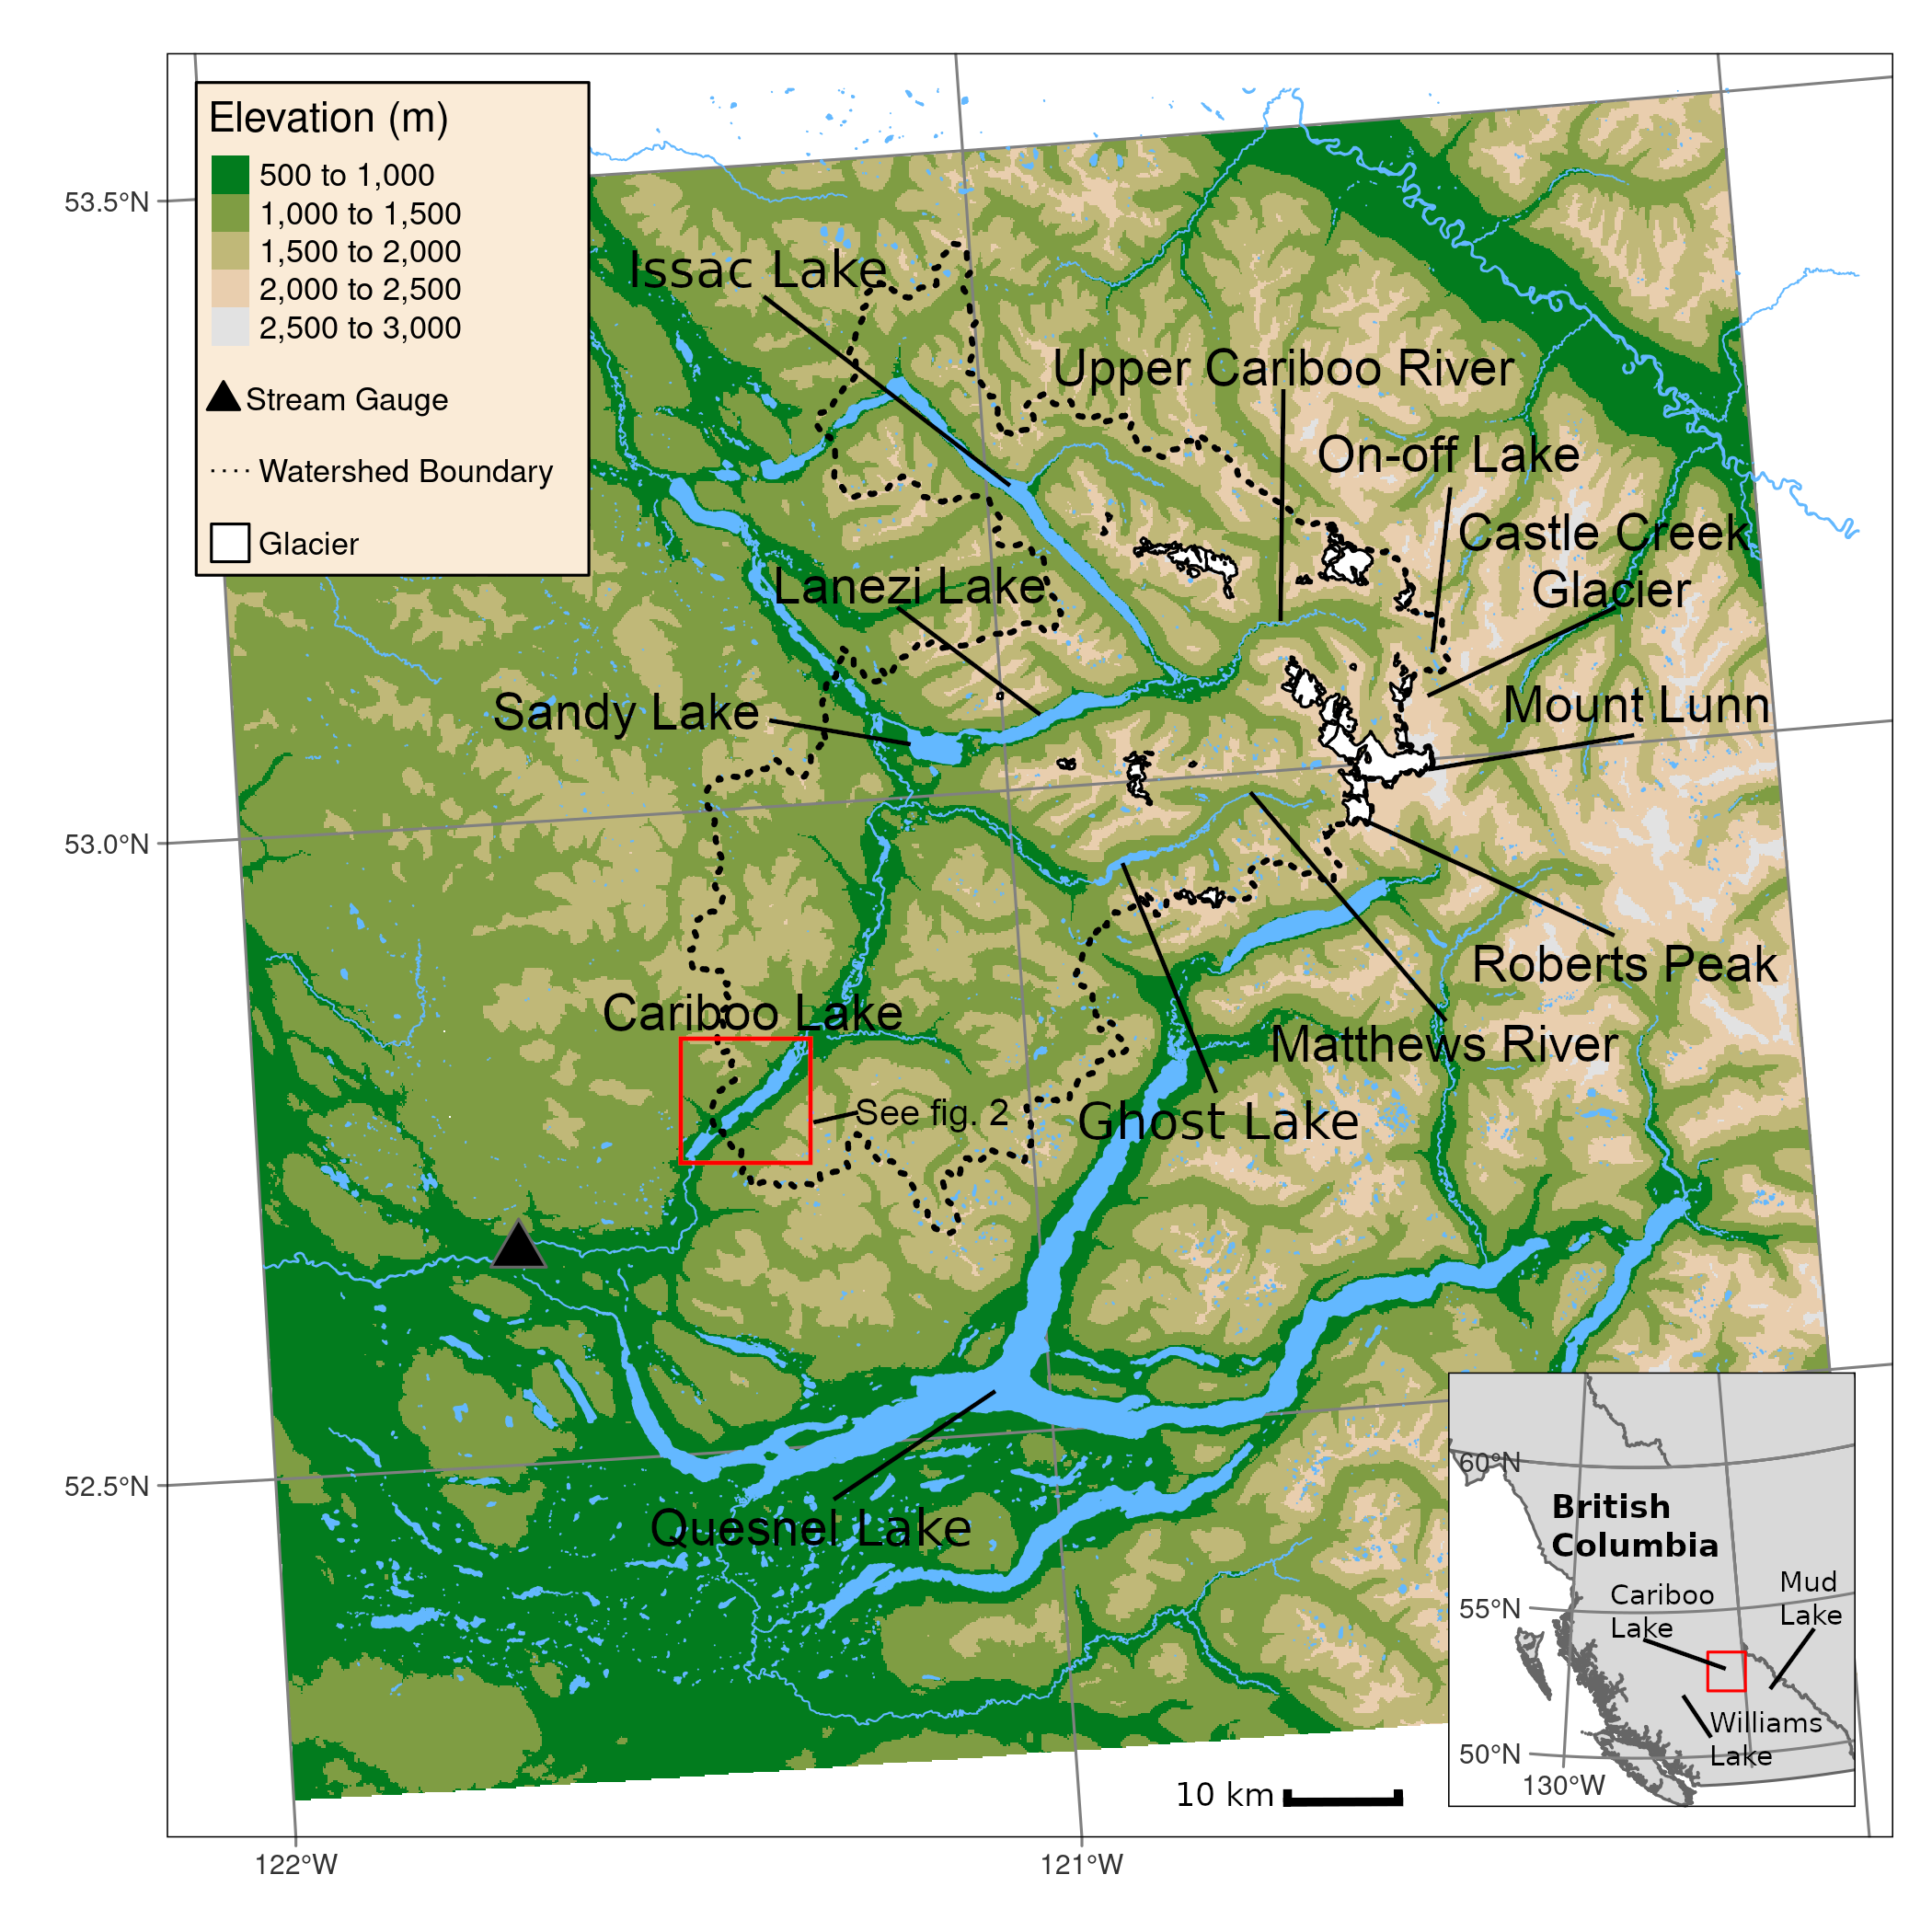
\includegraphics[width=0.95\textwidth,height=\textheight]{figs/cl_small_scale_inset_labels_gimp.png}

}

\caption{\label{fig-map-basin}\ldots{}}

\end{figure}

\begin{figure}

{\centering \includegraphics[width=1\textwidth,height=\textheight]{figs/cl_bathymetry_acoustics_coring_locations_labels.png}

}

\caption{\label{fig-map-lake}\ldots{}}

\end{figure}

\begin{figure}

{\centering 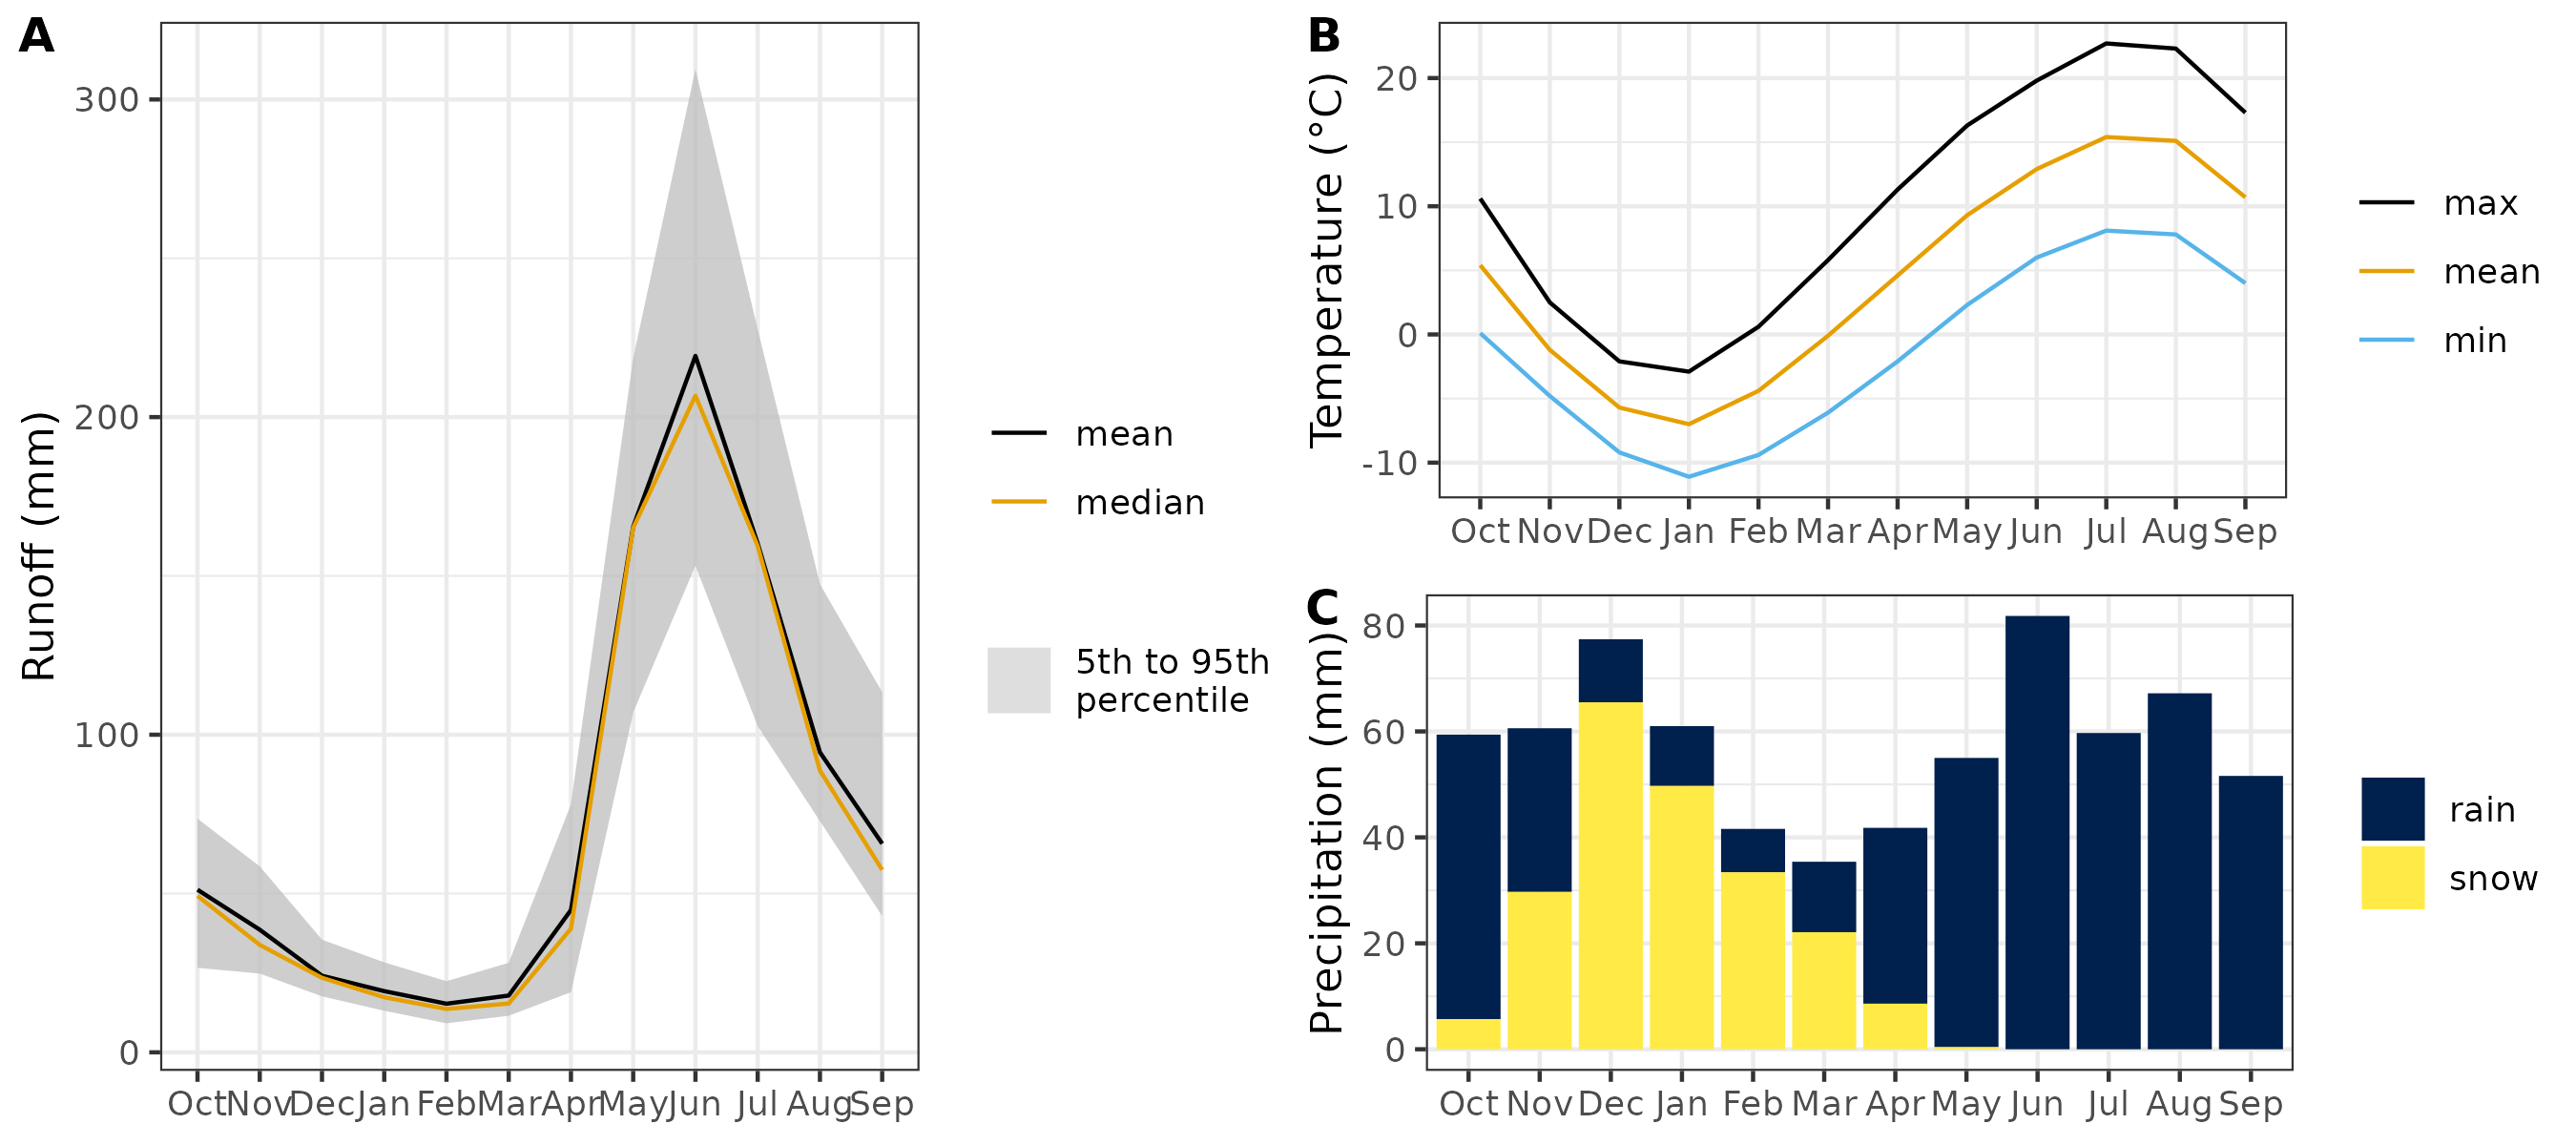
\includegraphics[width=1\textwidth,height=\textheight]{figs/cariboo_combine_climate_hydro.png}

}

\caption{\label{fig-cl-hydro}\ldots{}}

\end{figure}

\begin{figure}

{\centering \includegraphics[width=1\textwidth,height=\textheight]{figs/acoustics_6_panel_cjes.png}

}

\caption{\label{fig-acoustics}\ldots{}}

\end{figure}

\begin{figure}

{\centering 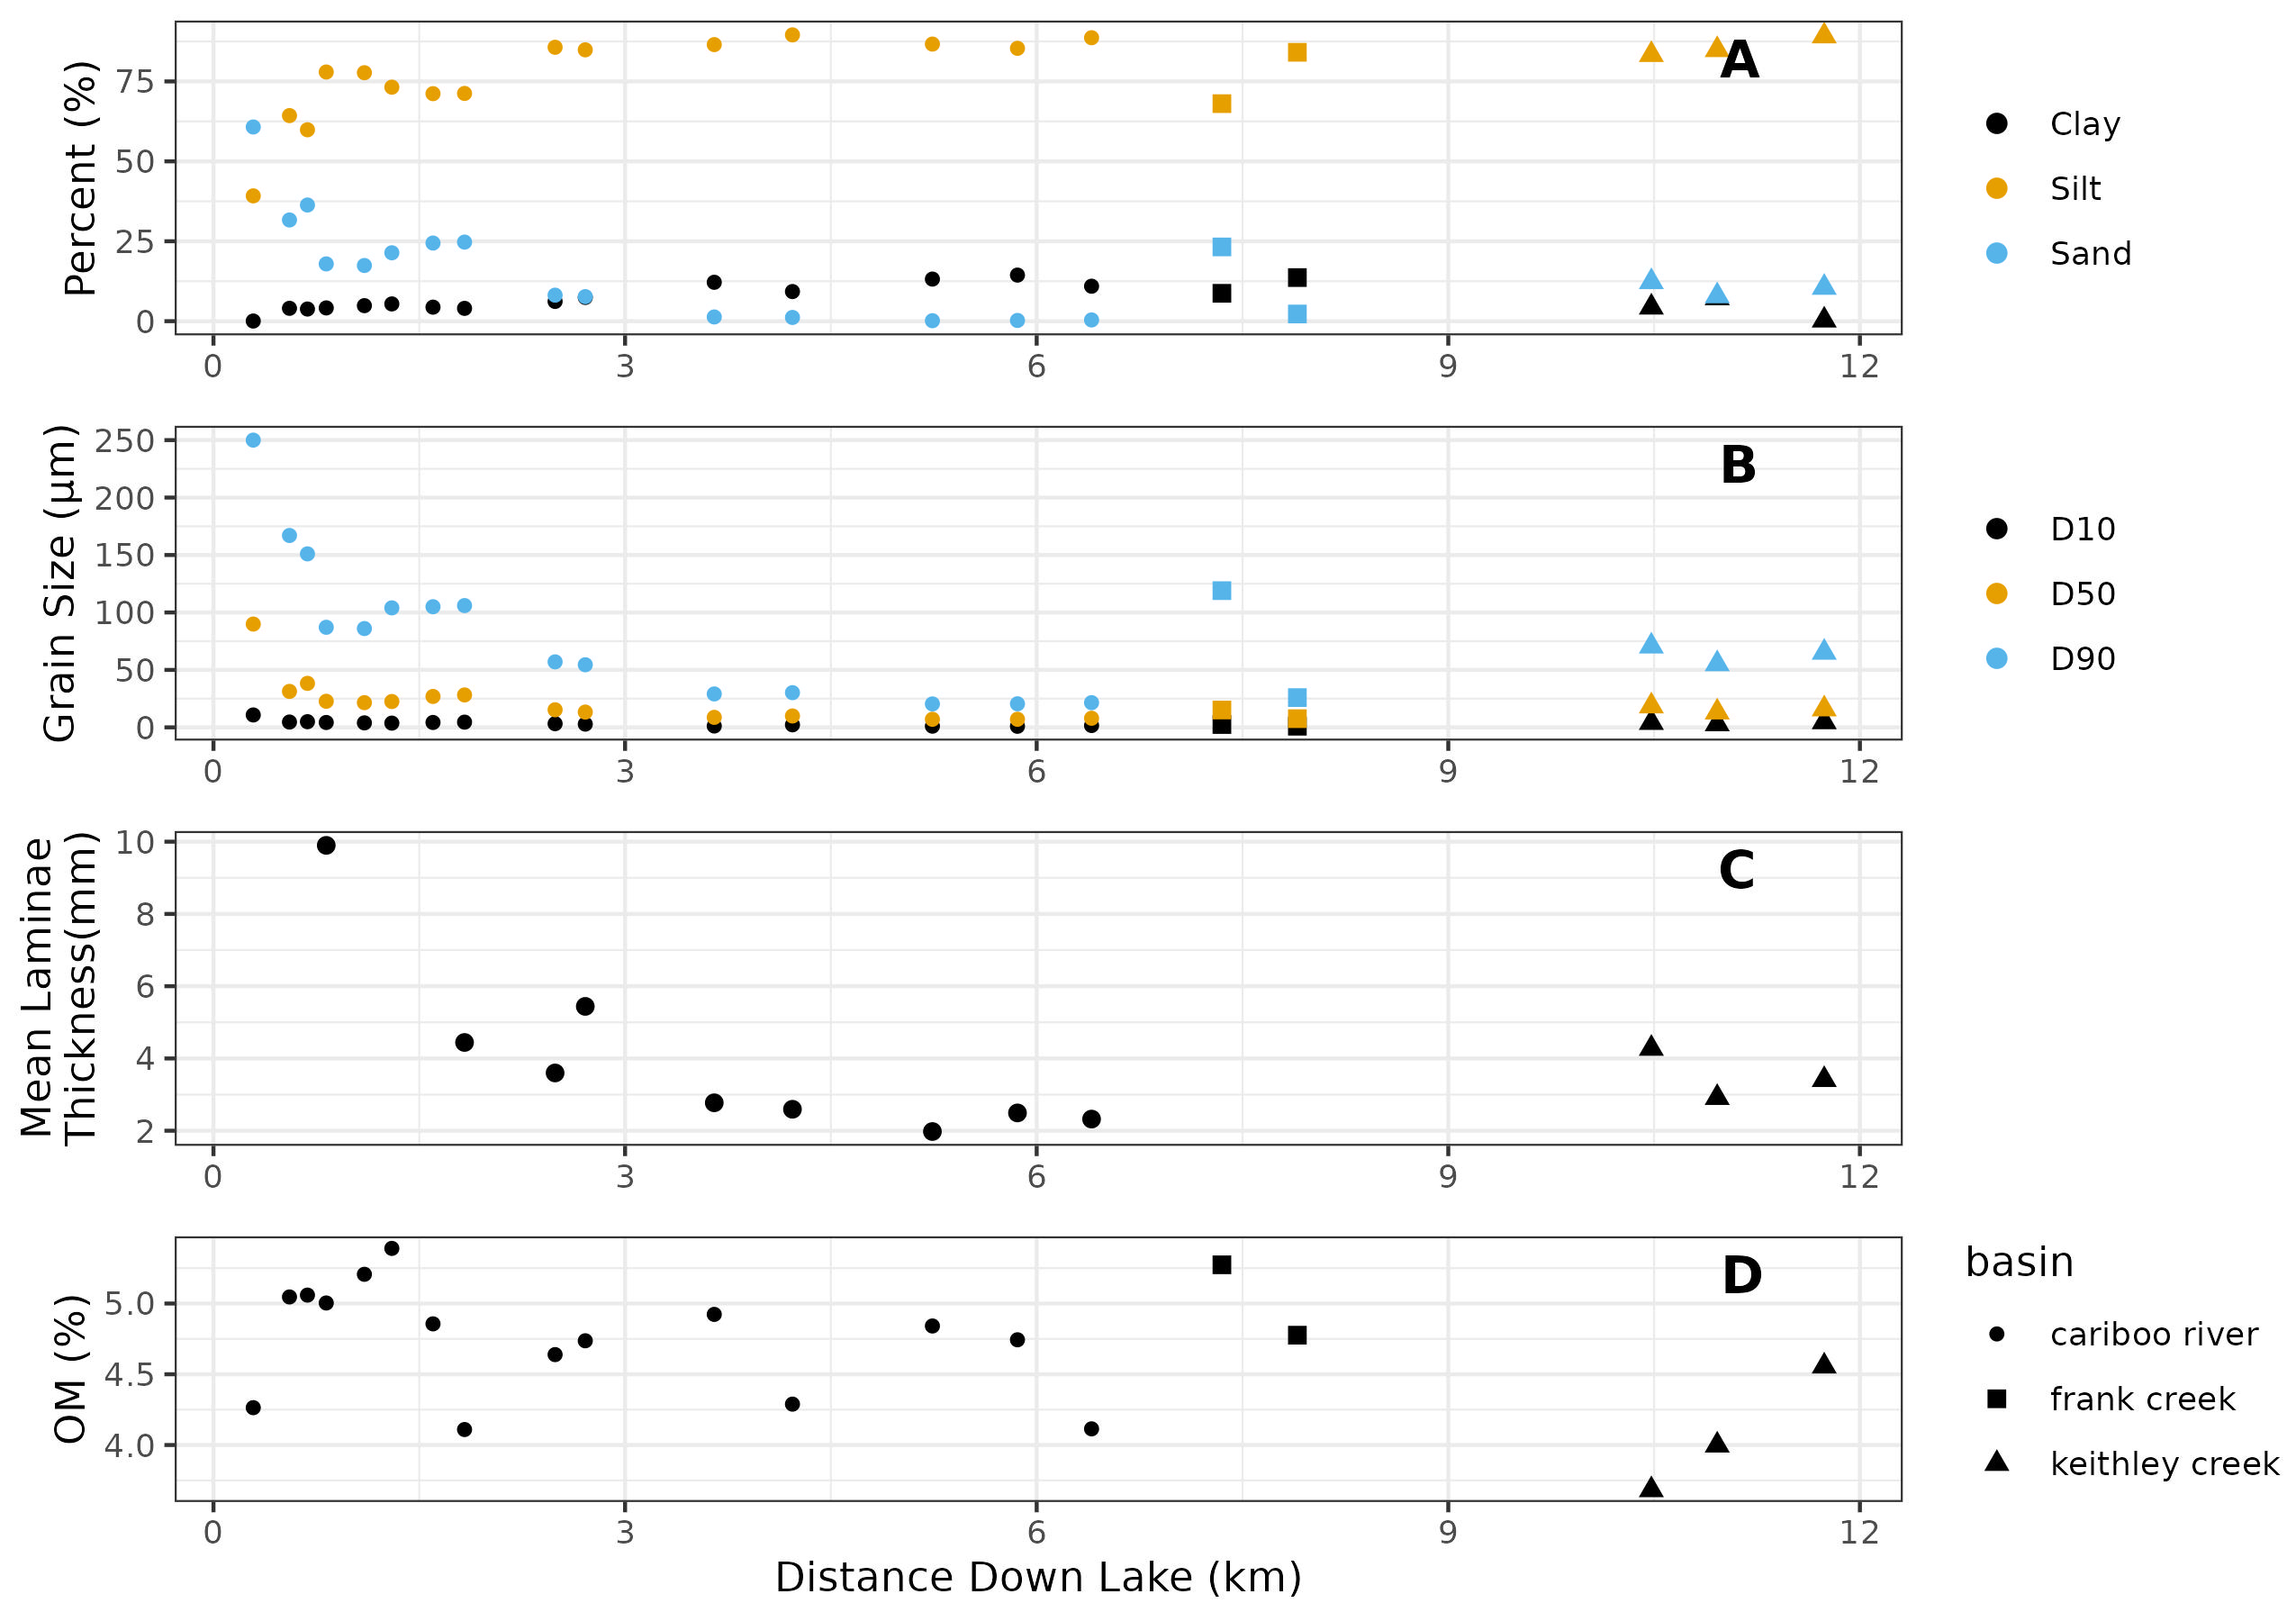
\includegraphics[width=1\textwidth,height=\textheight]{figs/ekman_seds.jpg}

}

\caption{\label{fig-ekmanSeds}\ldots{}}

\end{figure}

\begin{figure}

{\centering 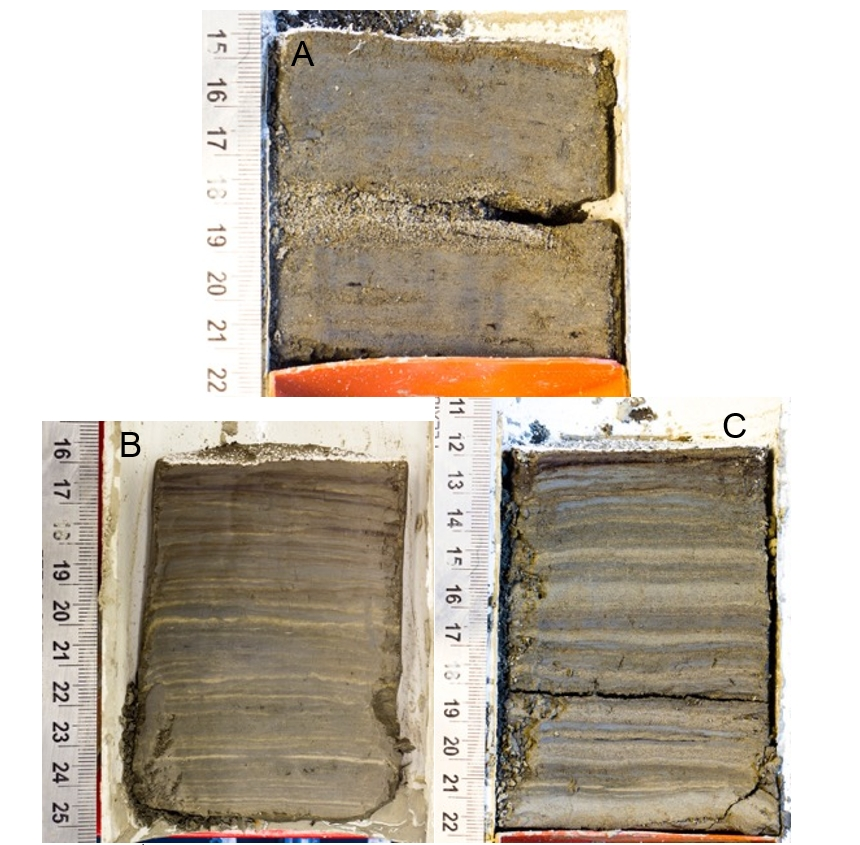
\includegraphics[width=1\textwidth,height=\textheight]{figs/ekman_example.jpg}

}

\caption{\label{fig-ekmanImgs}\ldots{}}

\end{figure}

\begin{figure}

{\centering 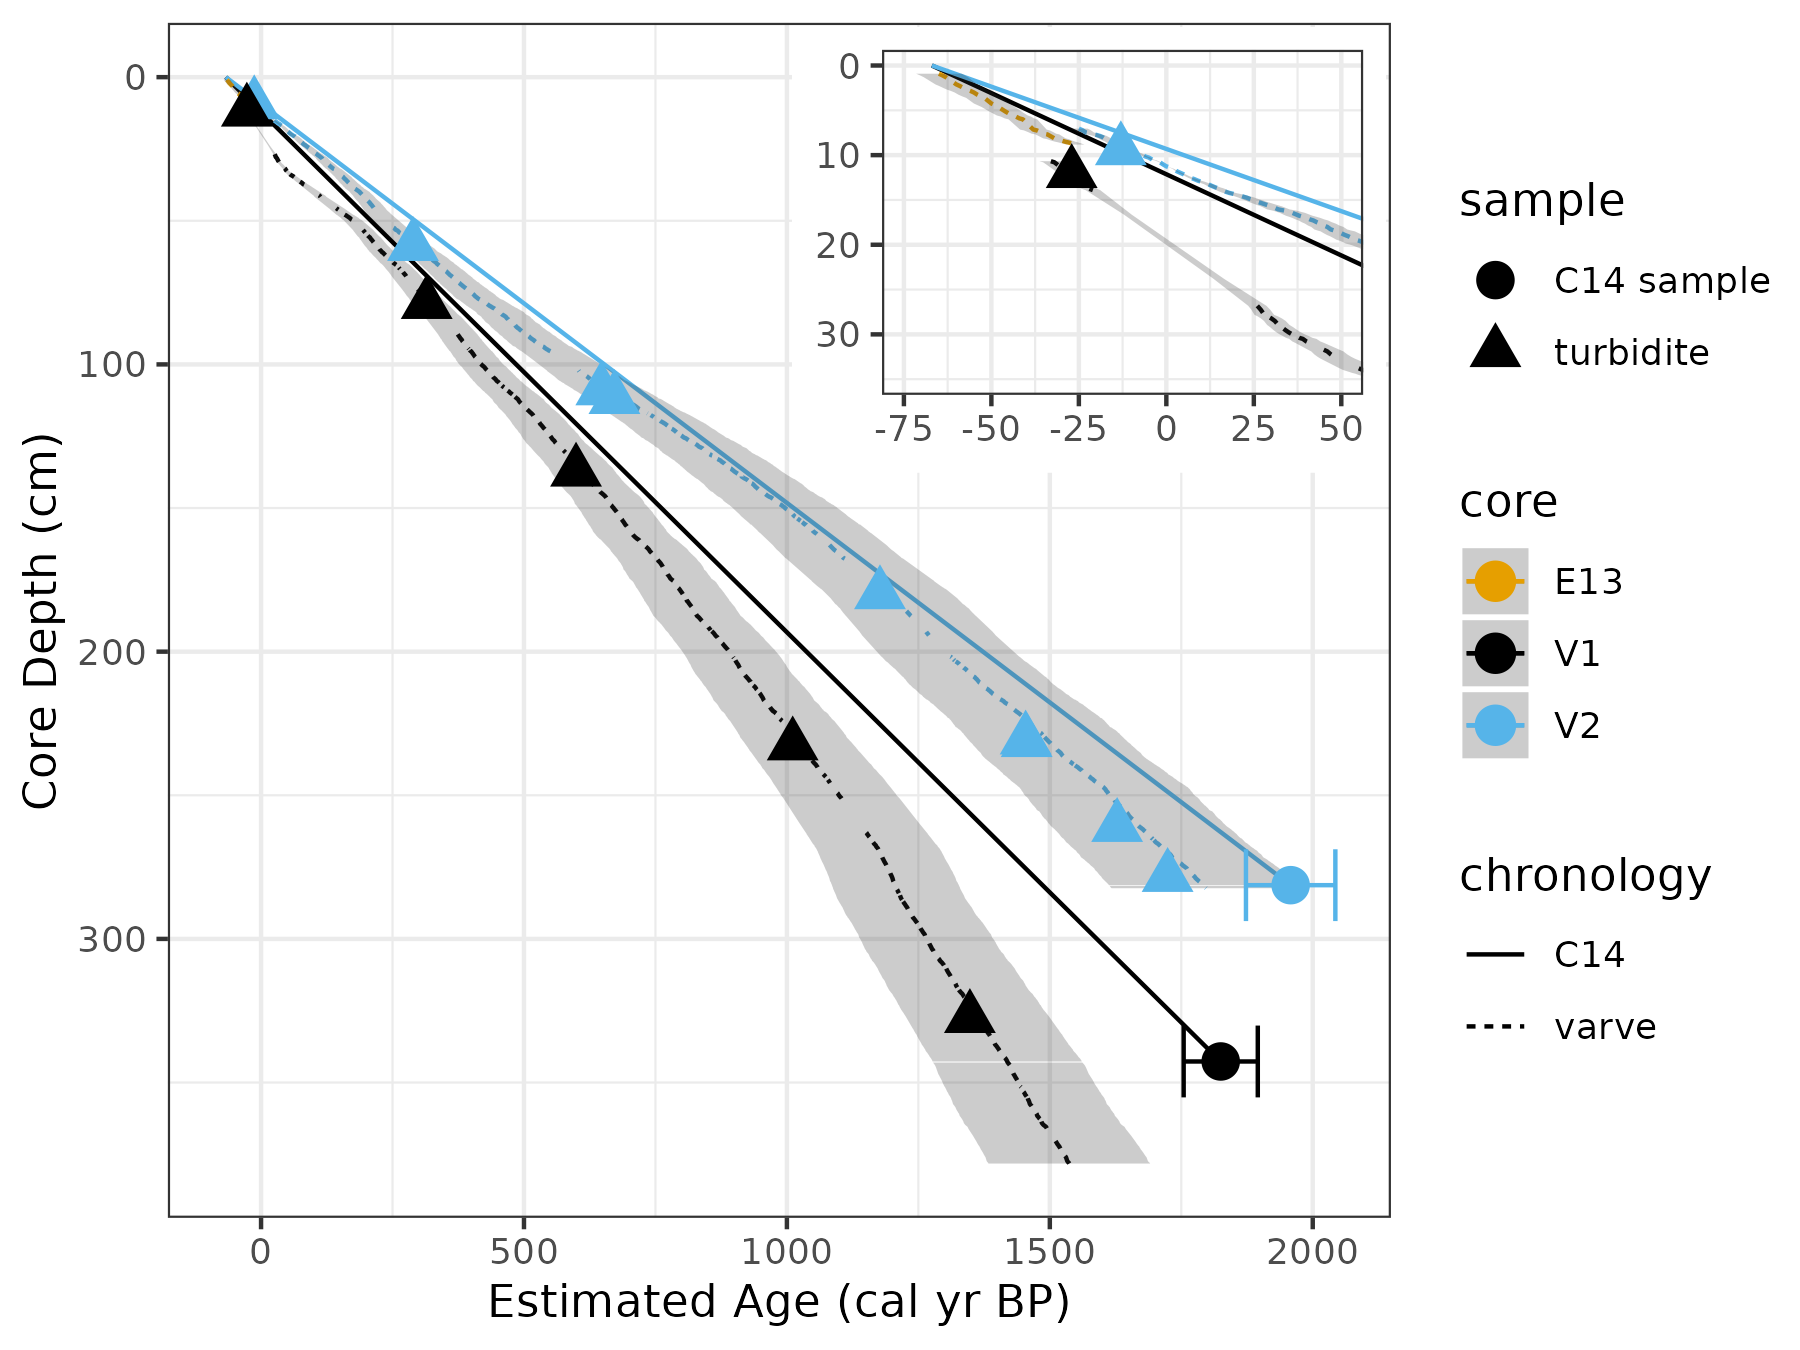
\includegraphics[width=1\textwidth,height=\textheight]{figs/longcore_cumulative_depth_vs_estimated_year_w_ams_and_varve.png}

}

\caption{\label{fig-amsRates}\ldots{}}

\end{figure}

\begin{figure}

{\centering 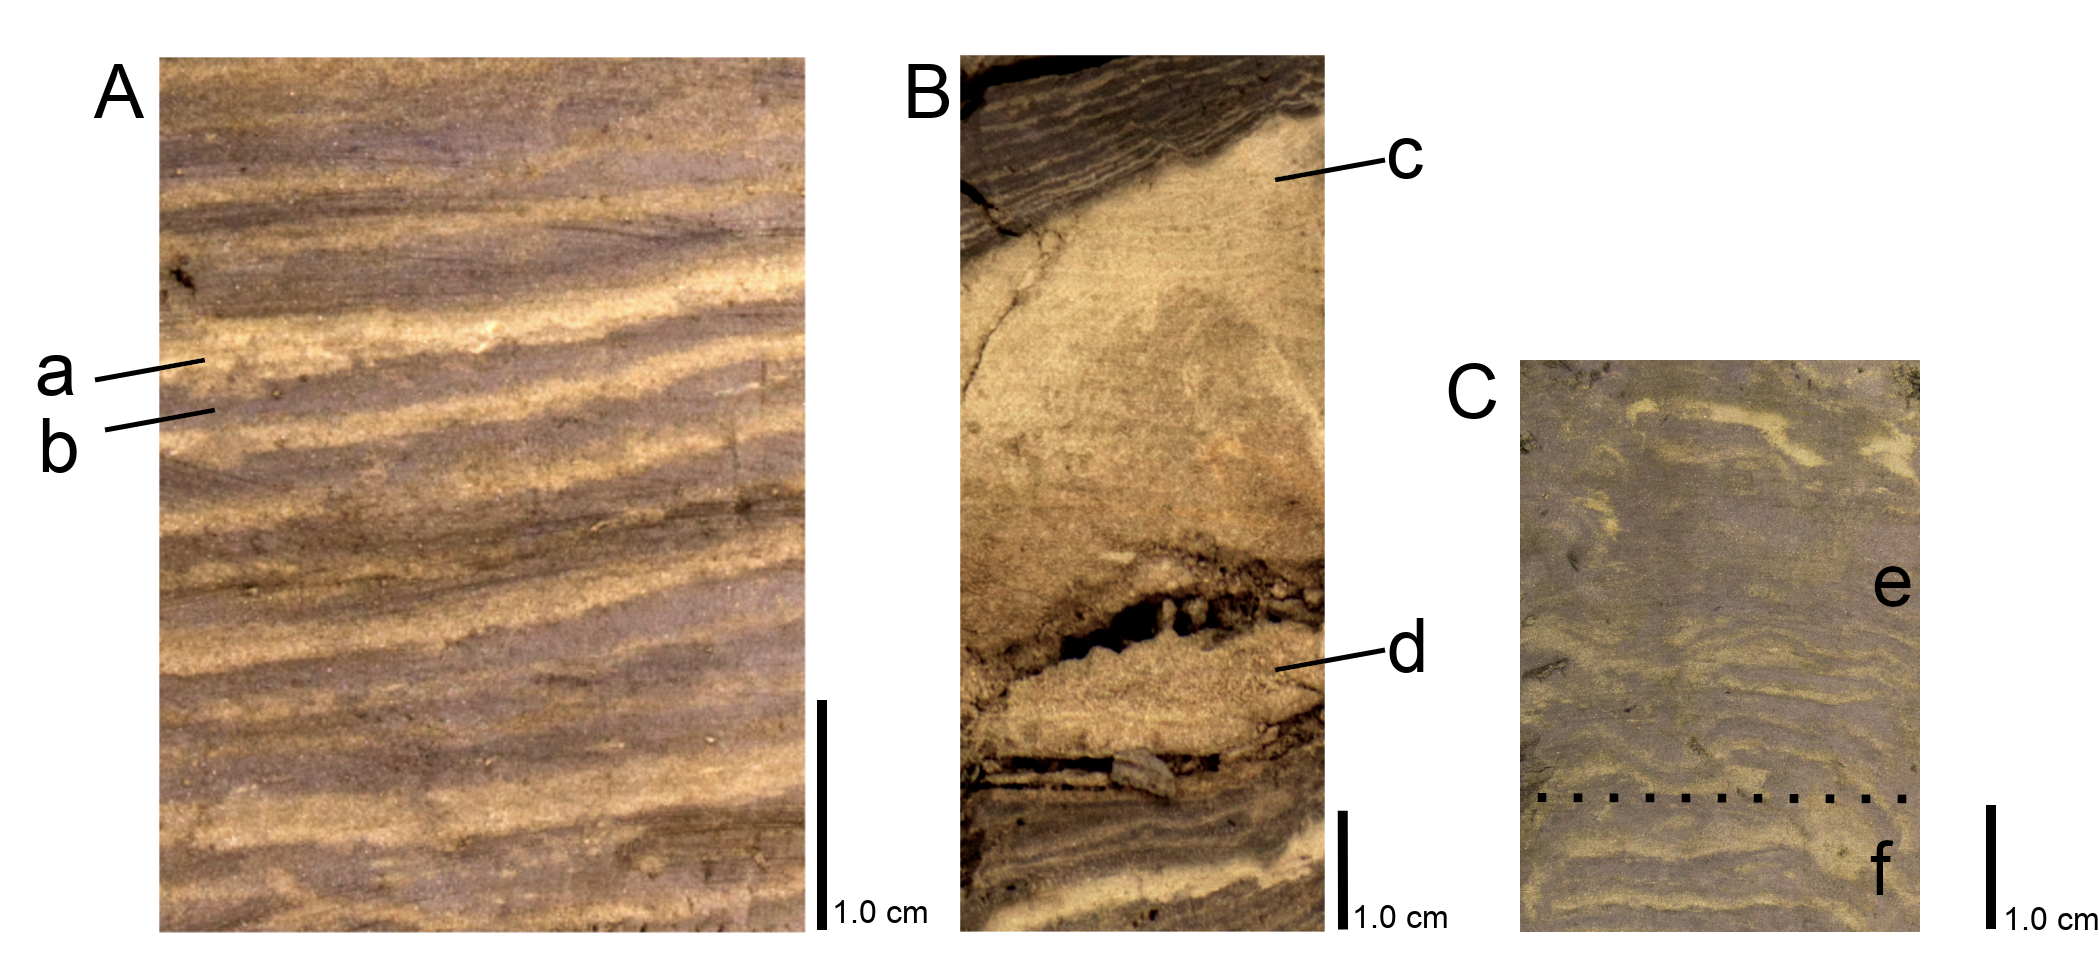
\includegraphics[width=1\textwidth,height=\textheight]{figs/good_vs_flood_vs_disturbed_varves_.png}

}

\caption{\label{fig-varve-turb}\ldots{}}

\end{figure}

\begin{figure}

{\centering 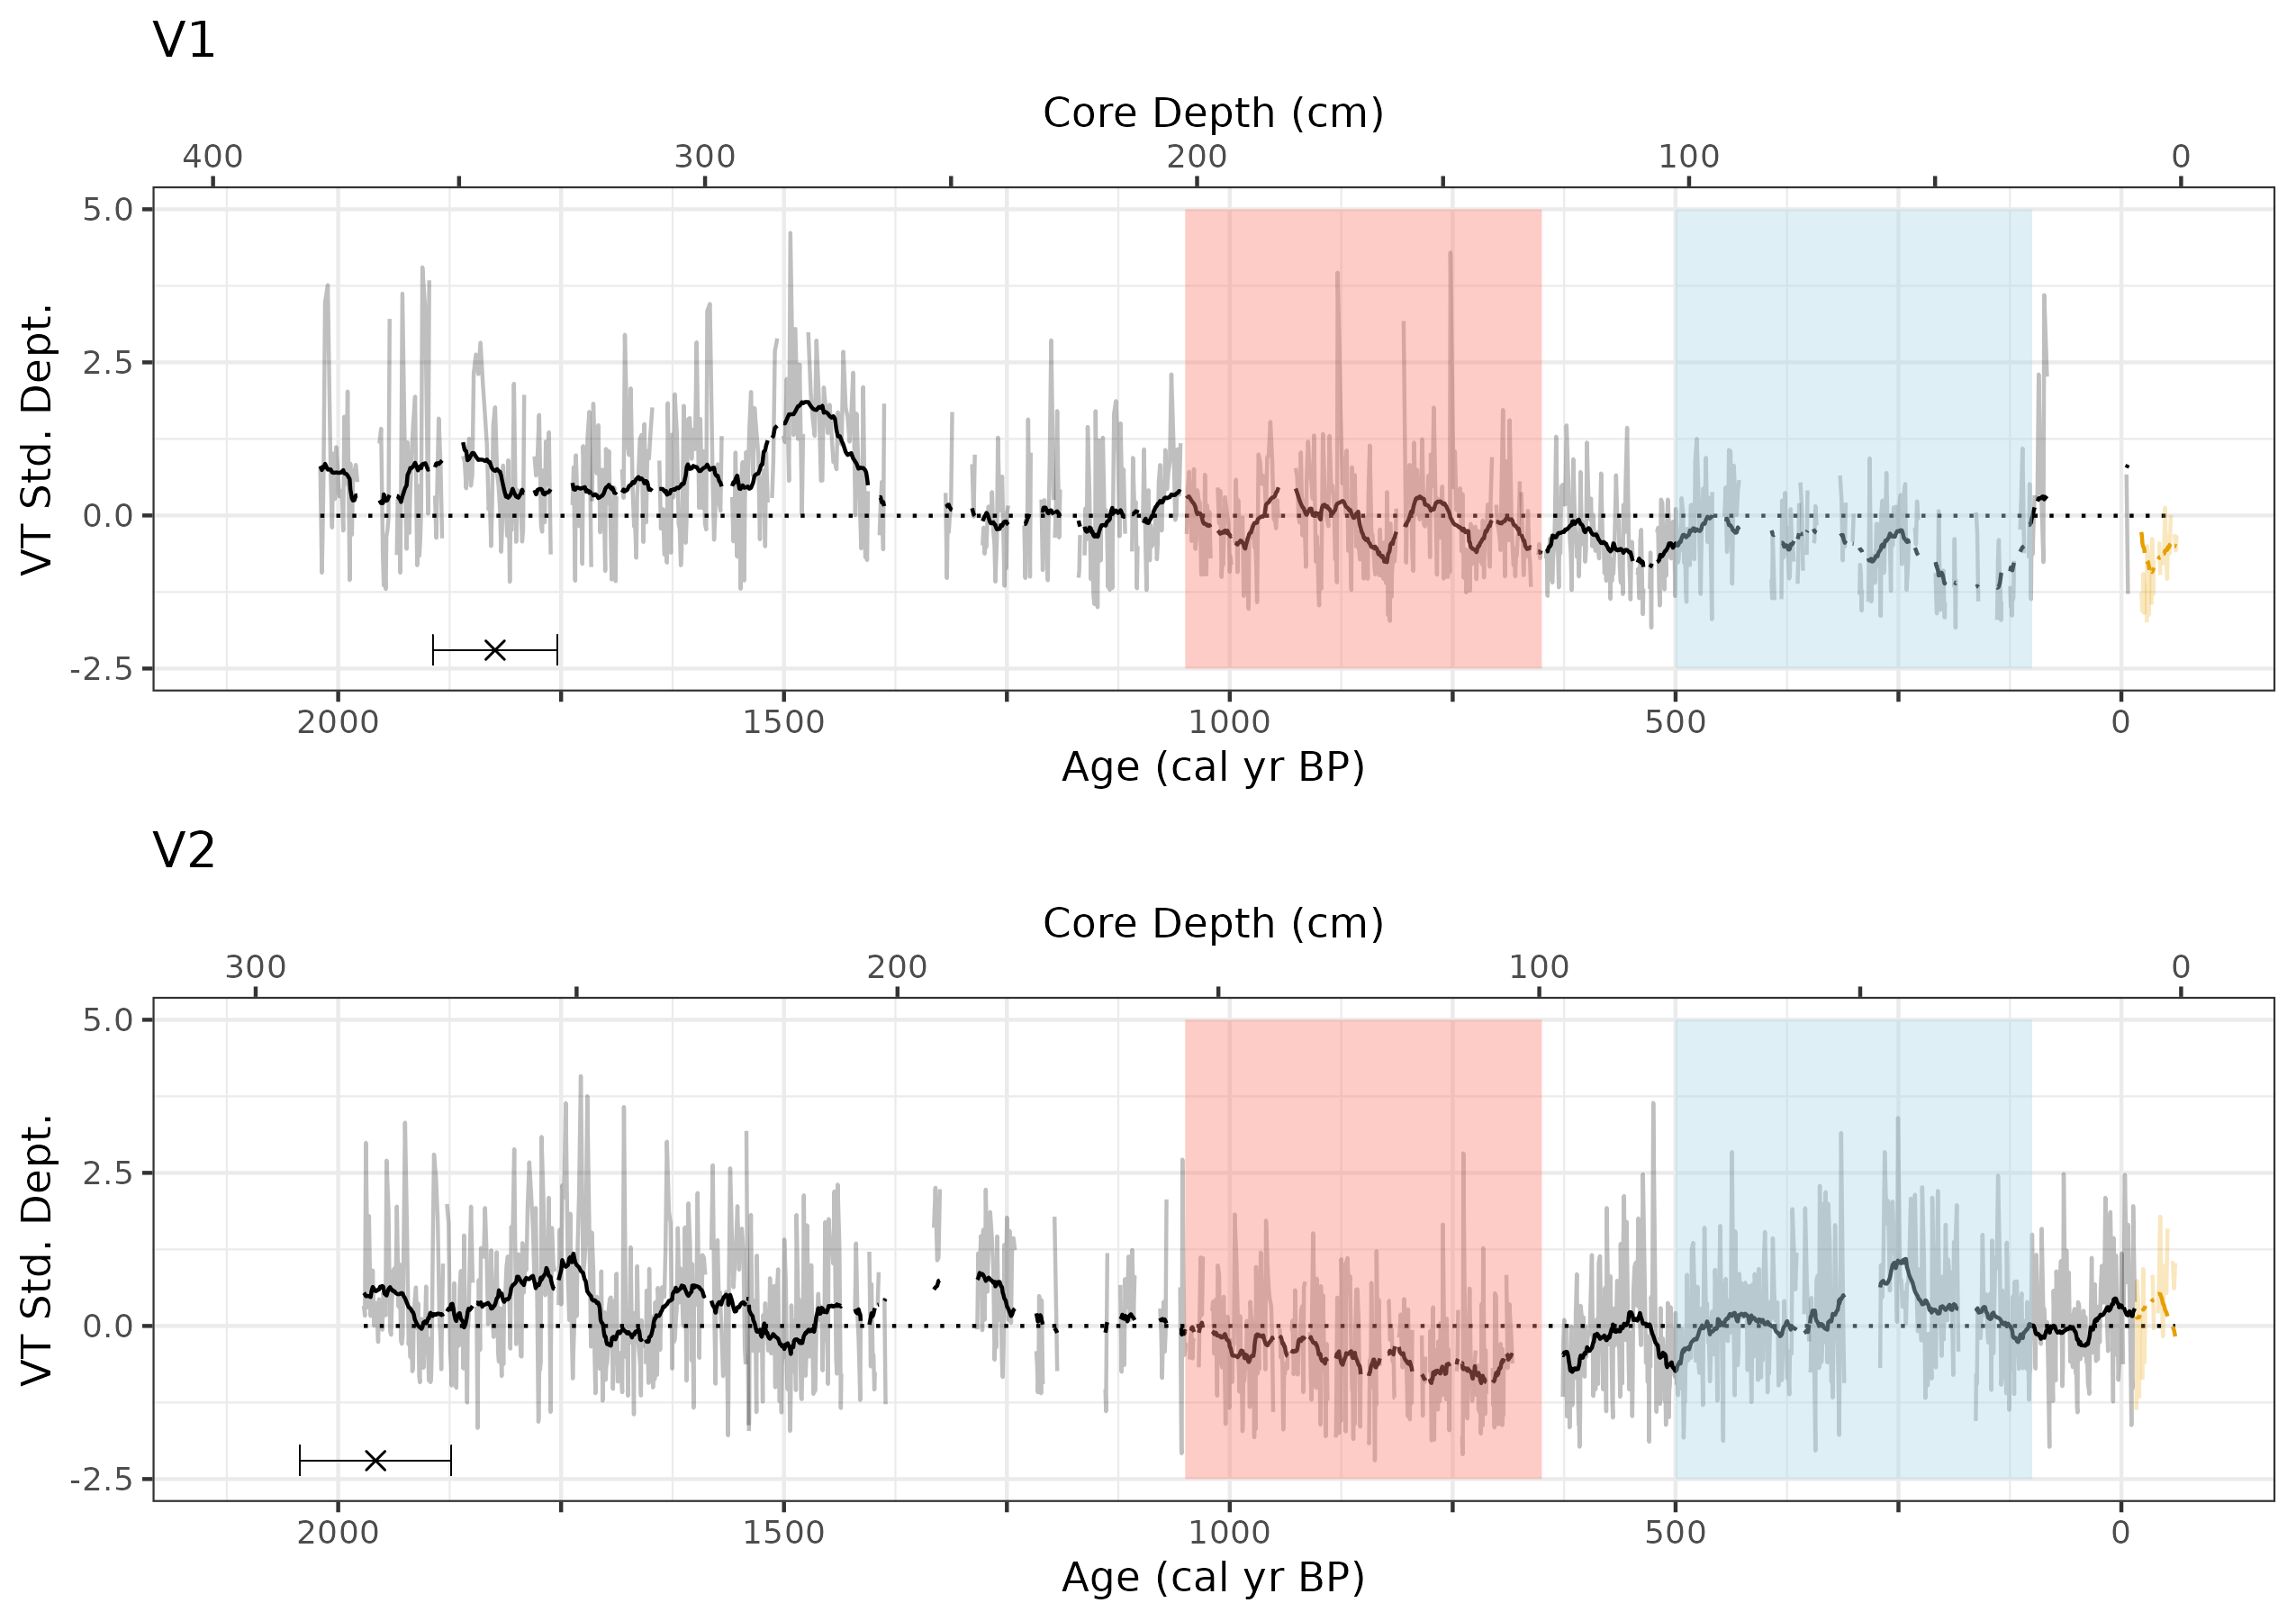
\includegraphics[width=1\textwidth,height=\textheight]{figs/V1_V2_varvethickness_vs_depth_and_C14_est_yr_ma.png}

}

\caption{\label{fig-varves-a}\ldots{}}

\end{figure}

\begin{figure}

{\centering 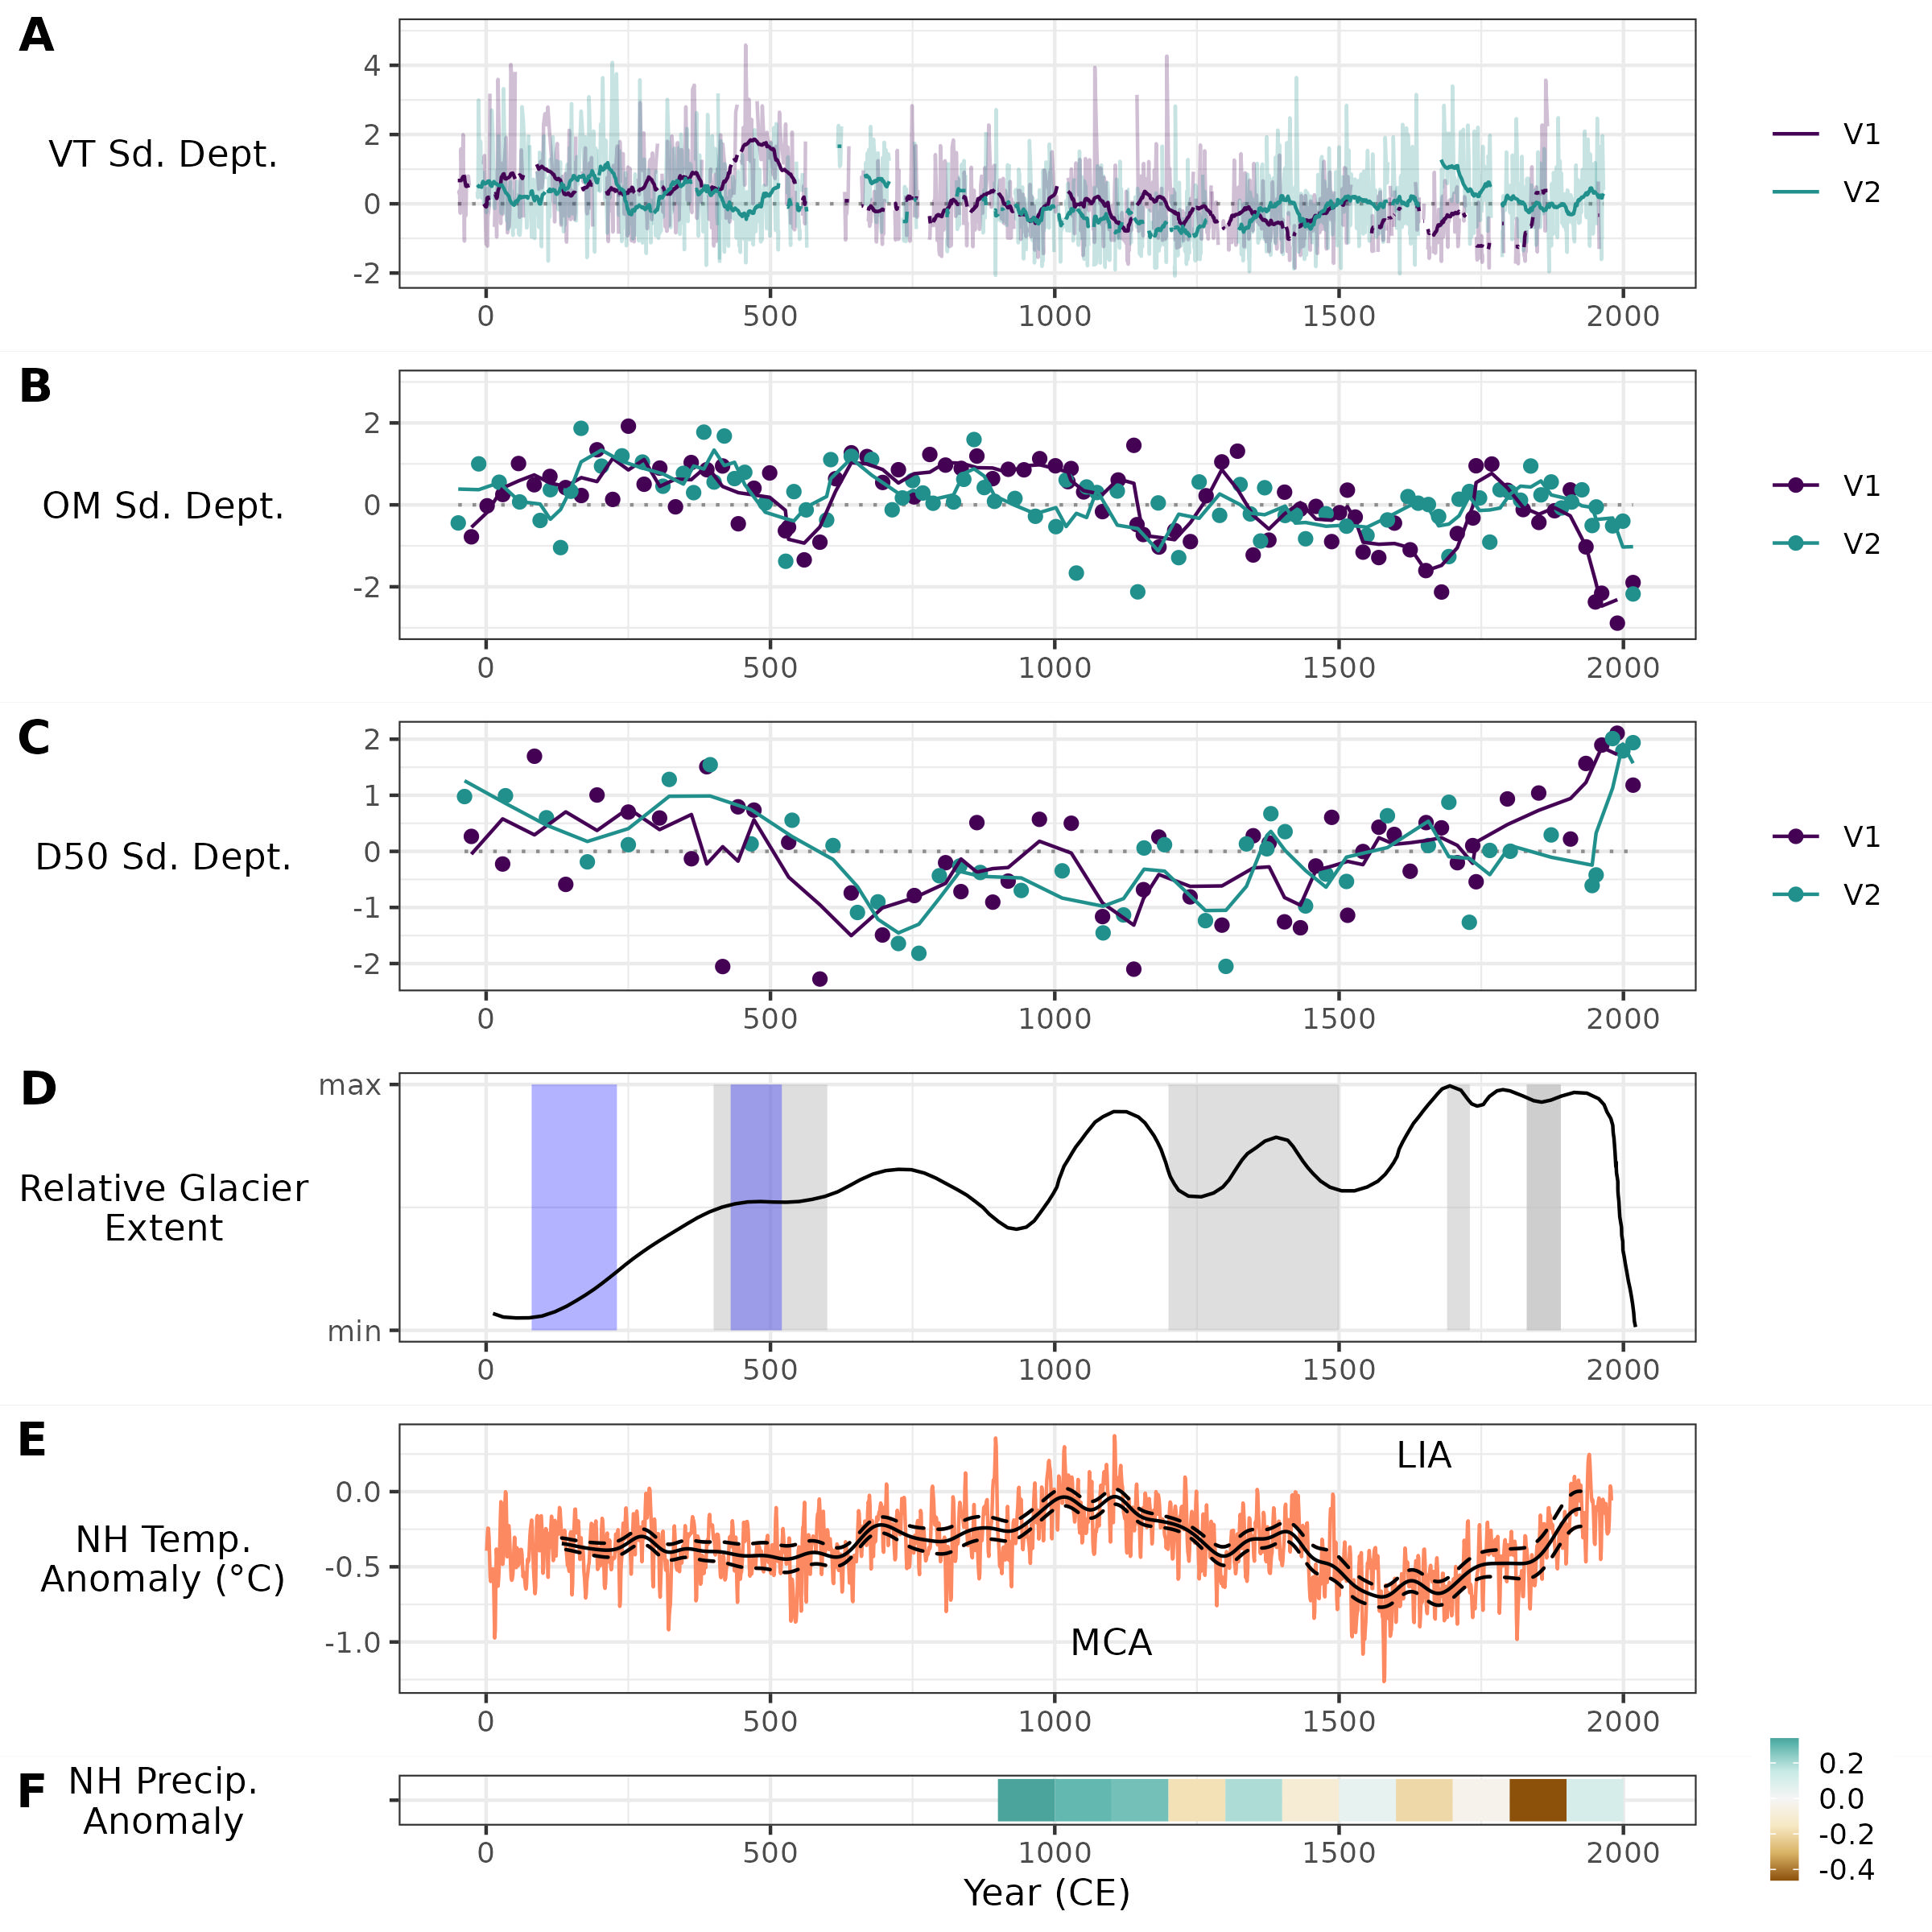
\includegraphics[width=1\textwidth,height=\textheight]{figs/all_core_stats_2k_anomalies.jpg}

}

\caption{\label{fig-proxy-comparison}\ldots{}}

\end{figure}

\pagebreak

\hypertarget{appendix}{%
\section{Appendix}\label{appendix}}

\hypertarget{tbl-ekErr}{}
\begin{table}
\caption{\label{tbl-ekErr}Counting error statistics from three Ekman short cores. }\tabularnewline

\centering
\begin{tabular}{r|r|r}
\hline
Core ID & Depth (cm) & Couplet Count\\
\hline
12 & 5 & 10\\
\hline
13 & 5 & 12\\
\hline
14 & 5 & 12\\
\hline
\end{tabular}
\end{table}



\end{document}
